\documentclass{article}

\usepackage[utf8]{inputenc}
\usepackage[italian]{babel}
\usepackage{wrapfig}
\usepackage{hyperref}
\usepackage{listings}
\usepackage{amsfonts} 
\usepackage[table]{xcolor}
\usepackage{makecell}
\usepackage[table]{xcolor}
\usepackage{enumerate}
\usepackage[shortlabels]{enumitem}
\renewcommand{\arraystretch}{1.4}
\usepackage{array, cellspace}
\setlength{\cellspacetoplimit}{4pt}
\setlength{\cellspacebottomlimit}{4pt}
\usepackage{graphicx}
\usepackage[export]{adjustbox} 
\usepackage{float}
\usepackage{
    geometry,
	plain,
	setspace,
	titlesec,
}

\geometry{
	paperheight = 29.7cm,
	paperwidth = 21cm,
	outer = 1.5cm,
	inner = 2.5cm,
	top = 2cm,
	bottom = 2cm
}
\singlespacing

\usepackage{blindtext}
\usepackage{nameref}

\newcounter{mylabelcounter}

\makeatletter
\newcommand{\labelText}[2]{%
#1\refstepcounter{mylabelcounter}%
\immediate\write\@auxout{%
  \string\newlabel{#2}{{1}{\thepage}{{\unexpanded{#1}}}{mylabelcounter.\number\value{mylabelcounter}}{}}%
}%
}
\makeatother

\begin{document}



\pagestyle{plain}
\thispagestyle{empty}

\graphicspath{{assets/figures/}}

\begin{center}
	\begin{figure}[h!]
		\centerline{
\includegraphics[width=0.6\textwidth]{Img/logo_unitn_black_center.eps}}
	\end{figure}

	\vspace{2 cm}

	\LARGE{Dipartimento di Ingegneria e Scienza dell’Informazione}

	\vspace{1 cm}

	\Large{
		Corso di Laurea in\\
		Informatica
	}

	\vspace{2 cm}
	\Large\textsc{Progetto Ingegneria del Software\\}
	\vspace{1 cm}
	\Huge\textsc{Sistema di monitoraggio ambientale\\}
	\vspace{1cm}
	\Large{D4 G19}

	\vspace{4cm}

	\Large{Anno accademico 2021/2022}
\end{center}
\tableofcontents
\section{Obiettivi}
Il progetto ha come obiettivo la realizzazione di un'applicazione compatibile con iOS e Android, in grado di gestire le prenotazioni dei parcheggi all’interno di un parcheggio di medio/grandi dimensioni registrati sull’applicazione.

In dettaglio l’applicazione deve permettere, ad un utente registrato ed autenticato, di:

\subsection{Cercare un parcheggio}
    All’interno di una determinata zona, sul navigatore. L’applicazione mostra i parcheggi con \textbf{colori} diversi a seconda della \textbf{disponibilità} dei posti. L’utente può selezionare il parcheggio desiderato e \textbf{prenotare} un posto, pagando tramite carta di credito o wallet integrato nell'applicazione;
\subsection{Gestire le prenotazioni}
    Quando una prenotazione viene confermata dall’applicazione la \textbf{targa} della macchina viene inviata all'infrastruttura del parcheggio in modo da consentirne l’accesso al suo arrivo. Condizione necessaria per confermare la prenotazione è che sul wallet o sulla carta di credito \textbf{ci siano i soldi necessari};
\subsection{Ingresso nel parcheggio}
    Una volta arrivati al parcheggio la sbarra si alza automaticamente, in quanto una videocamera legge e controlla se sono state effettuate prenotazioni con una determinata targa;
\subsection{Aggiungi parcheggi}
    In particolare, se un utente è il \textbf{proprietario di un parcheggio} non registrato può richiedere il servizio compilando un form integrato nell’applicazione, dove dovrà indicare i dati del parcheggio: nome, via, numero civico, città, cap, posti disponibili e attestare la proprietà tramite un documento.
    Una volta verificata l’autenticità dei dati sull’account dell’utente verranno attivate le funzionalità per gestire il parcheggio, tra cui: \textbf{analytics} e possibilità di \textbf{sospendere il servizio temporaneamente}. \newline\\
Nel caso in cui un utente non registrato volesse richiedere l’attivazione del servizio, perché proprietario di un parcheggio, può indicarlo al momento della registrazione (compilando i campi indicati nel punto 4).
\section{Requisiti Funzionali}

\subsection{Requisiti generali:}
\label{Requisiti generali}
\begin{itemize}
    \item L’applicazione SMART PARKING dovrà essere un’app per \textbf{smartphone};
    \item l’applicazione deve essere composta da una schermata principale dove poter \textbf{cercare i parcheggi} e un \textbf{menù ad hamburger};
    \item Il sistema deve avere 3 livelli di accesso:
    \begin{itemize}
        \item Utente \textbf{non registrato};
        \item Utente \textbf{registrato ed autenticato};
        \item Utente \textbf{proprietario di parcheggio};
    \end{itemize}
    \item il sistema deve mostrare la \textbf{situazione generale} dei parcheggi in base alla disponibilità
    \item Il sistema deve gestire le \textbf{prenotazioni};
    \item Il sistema deve gestire i pagamenti tramite \textbf{wallet/carta di credito};
\end{itemize}

\subsection{Utenti}
\subsection*{Utente non registrato/non autenticato}

\begin{enumerate}[start=1,label={\bfseries RF\arabic*}]
    \item \label{itm:RF1} L’utente non registrato può selezionare se \textbf{registrarsi} come “utente” o “proprietario di parcheggio”:
    \begin{itemize}
        \item se l’utente seleziona “\textbf{utente}” il sistema chiede di inserire: i suoi dati personali (nome, cognome, data di nascita, CF, email, numero di telefono) ed una password (da confermare due volte) oppure può registrarsi utilizzando un account google, facebook o apple.
        Una volta inseriti i dati, il sistema invia una mail contenente un link di conferma all’indirizzo specificato. Nel caso l’utente non ricevesse la mail può cliccare su un tasto per chiedere che gli sia inviata nuovamente.
        \item se l’utente seleziona “\textbf{proprietario di parcheggio}” il sistema chiede di inserire i dati personali del proprietario del parcheggio, i dati del parcheggio, ovvero, nome del parcheggio, via, città, cap, posti disponibili, le varie tariffe (oraria, giornaliera) e i giorni in cui il parcheggio è a pagamento;
    \end{itemize}
    \item \label{itm:RF2} Se l’utente non autenticato non si ricorda la password può richiederne il \textbf{reset}, inserendo l’email verificata collegata all’account in modo da ricevere una mail che contiene un link per cambiare la password. L’utente dovrà inserire la nuova password e confermare. 
\end{enumerate}

\subsection*{Utente autenticato}
\begin{enumerate}[start=3,label={\bfseries RF\arabic*}]
    \item \label{itm:RF3} Per effettuare il login l’utente dovrà inserire \textbf{email} e \textbf{password}. Nel caso l’account non esista appare un messaggio di errore, cancellando il contenuto del campo password.
    \item \label{itm:RF4} Dopo il primo login all’utente verrà chiesto di inserire anche: un \textbf{metodo di pagamento attivo} (carta di credito) e la \textbf{targa} delle macchine che vuole utilizzare. È obbligatorio compilare almeno una volta il metodo di pagamento e la targa;
    \item \label{itm:RF5}Composizione del menù: l’utente autenticato ha a disposizione un \textbf{menù ad hamburger} dove può effettuare le seguenti operazioni:
    \begin{itemize}
        \item \textbf{cercare i parcheggi} (sezione principale) sulla mappa di Google maps;
        \item \textbf{visualizzare dati personali} e \textbf{modificare}: email, numero di telefono, elenco delle carte di credito, lista delle targhe;
        \item \textbf{visualizzare} la disponibilità del \textbf{wallet}, ricaricarlo e l’elenco delle \textbf{transazioni effettuate};
        \item \textbf{visualizzare e gestire le prenotazioni effettuate};
        \item \textcolor{red}{passare all'account "\textbf{parcheggiatore}"};
        \item \textbf{logout} dall’appliazione: quando si preme questa voce il sistema ti riporta alla schermata di login.
    \end{itemize}
    \item \label{itm:RF6}L’utente autenticato può cercare i parcheggi con posti disponibili, con la possibilità di utilizzare un \textbf{filtro} per:
    \begin{itemize}
        \item selezionare il \textbf{raggio} in cui cercare i parcheggi;
        \item selezionare la \textbf{tariffa oraria massima};
        \item parcheggi \textbf{preferiti}.
    \end{itemize}
    \subitem I parcheggi verranno mostrati sulla mappa con \textbf{3 colori in base alla disponibilità}: rosso, arancione, verde.
    \item \label{itm:RF7} Una volta che l’utente ha cercato i parcheggi è possibile \textbf{ordinarli} per:
    \begin{itemize}
        \item tariffa oraria;
        \item distanza dalla posizione;
        \item disponibilità posti;
        \item ordine alfabetico.
    \end{itemize}
    \item \label{itm:RF8}L’utente autenticato può prenotare un posto nel parcheggio selezionandolo dalla mappa. L’utente deve anche selezionare la \textbf{targa} della macchina con cui si recherà nel parcheggio, il \textbf{giorno} in cui vuole prenotare (se sosta per più di 24h) e per \textbf{quanto} vuole sostare nel parcheggio;
    \item \label{itm:RF9}L'utente autenticato può \textbf{aggiungere} un parcheggio nella lista dei \textbf{preferiti};
    \item \label{itm:RF10}L’utente autenticato può \textbf{aggiungere nuovi metodi di pagamento} cliccando su \textcolor{red}{“modifica”} nella sezione dei suoi dati personali.
    \item \label{itm:RF11}L’utente \textcolor{red}{deve} selezionare una carta da utilizzare come \textcolor{red}{principale};
    \item \label{itm:RF12}L’utente autenticato può \textbf{modificare la password} aprendo il menù ad hamburger e selezionando \textcolor{red}{“dati personali”, "modifica"} inserendo la vecchia password e confermando la nuova due volte;
\end{enumerate}

\subsection*{Propietario parcheggio}
\begin{enumerate}[start=13,label={\bfseries RF\arabic*}]
    \item \label{itm:RF13}Il proprietario del parcheggio può gestire il suo parcheggio attraverso una schermata apposita selezionabile nel menù ad hamburger; 
    \item \label{itm:RF14}Il proprietario può \textbf{cambiare il costo per ora} del suo parcheggio;
    \item \label{itm:RF15}Il proprietario può \textbf{aggiungere nuove \textcolor{red}{aree parcheggio}} al suo account;
    \item \label{itm:RF16}Il proprietario può accedere ad una schermata di \textbf{analytics}, dove viene mostrato l’andamento del parcheggio selezionato, come: 
    \begin{itemize}
        \item \textbf{guadagni} mensili/semestrali/annuali;
        \item \textbf{istogramma} che mostra il numero di macchine parcheggiate al mese (12 mesi);
        \item il numero di \textbf{utenti} che hanno utilizzato il parcheggio \textbf{tramite l’applicazione}.
    \end{itemize}
    \item \label{itm:RF17}Il proprietario del parcheggio può \textbf{disiscriversi} dall’applicazione.
\end{enumerate}

\subsection{Gestione prenotazioni}
\begin{enumerate}[start=18,label={\bfseries RF\arabic*}]
    \item \label{itm:RF18} Il sistema deve permettere all’utente di prenotare il parcheggio selezionandolo e inserendo:
    \begin{itemize}
        \item \textbf{data} in cui desidera effettuare la prenotazione;
        \item \textbf{fascia oraria}.
    \end{itemize}
    \item \label{itm:RF19}In caso di prenotazione avvenuta con successo, \textcolor{red}{il parcheggio scala il numero di posti disponibili come descritto nell'\textbf{\nameref{label:RNF12}}};
    \item \label{itm:RF20}La prenotazione del parcheggio si suddivide in \textbf{due macro-categorie}, per lunghezza della prenotazione:
    \begin{itemize}
        \item \textbf{$<$ 24h}: l’utente ha \textbf{30 minuti} per arrivare al parcheggio una volta avvenuta la prenotazione, altrimenti la prenotazione del posto decade.
        \item \textbf{$>$ 24h}: l’utente \textbf{non ha un tempo limite} per arrivare al parcheggio. In questo caso l’utente può entrare ed uscire liberamente dal parcheggio finché non passa il tempo dichiarato inizialmente.
    \end{itemize}
    \item \label{itm:RF21}Il sistema deve permettere di annullare la prenotazione:
    \begin{itemize}
        \item prenotazione \textbf{$<$ 24h}: l’utente ha \textbf{20 minuti} per annullare la prenotazione (viene restituita la cauzione);
        \item prenotazione \textbf{$>$ 24h}: l’utente può annullare la prenotazione (ricevendo il rimborso) entro le \textbf{12h} precedenti l’effettiva prenotazione.
    \end{itemize}
\end{enumerate}

\subsection{Gestione pagamenti}
\begin{enumerate}[start=22,label={\bfseries RF\arabic*}]
    \item \label{itm:RF22} L’utente può caricare il wallet mediante carta di credito nel sottomenù “wallet”.
    \item \label{itm:RF23} Al momento della prenotazione se il wallet è pari o minore di 0 il sistema dovrà controllare la validità della carta di credito. Nel caso in cui la carta di credito non fosse valida la prenotazione verrà annullata.
    \item \label{itm:RF24} Pagamento suddiviso in base alla durata della prenotazione:
    \begin{itemize}
        \item \textbf{$<$ 24h}: Al momento del pagamento viene chiesta una cauzione di 2€, che verrà restituita se l’utente arriva al parcheggio in tempo.
        Quando l’utente arriva al parcheggio, la sbarra si alza senza dover prendere il biglietto (il sistema riconosce la targa). All’uscita la sbarra si alza e viene calcolata la tariffa dovuta, data da \textbf{\textit{tempo passato nel parcheggio} $\cdot$ \textit{tariffa oraria}}. La cauzione viene restituita e si detrae la tariffa dal wallet. Nel caso in cui l’importo da pagare sia maggiore del saldo del wallet, la differenza, più il 5\% del prezzo totale viene detratta dalla carta di credito registrata e collegata all’account.
        \item \textbf{$>$ 24h}: il pagamento della tariffa avviene al momento della prenotazione. Nel caso in cui l’utente lasci la macchina all’interno del parcheggio per più tempo di quanto dichiarato, all’uscita dal parcheggio dalla carta di credito viene addebitata la seguente tariffa: \textcolor{red}{\textbf{\textit{$($tempo $\cdot$ tariffa oraria$)-($costo già addebitata+5$\%$~costo già addebitato$)$.}}}
    \end{itemize}
\end{enumerate}

\section{Requisiti Non funzionali}

\textbf{\labelText{RNF1}{label:RNF1}. Compatibilità}
\begin{itemize}
    \item L’app deve funzionare su iOS (9 o superiori) e Android 7 (o superiori); 
\end{itemize}
\textbf{\labelText{RNF2}{label:RNF2}. Localizzazione}
\begin{itemize}
    \item \textcolor{red}{Il sistema utilizza il GPS del dispositivo};
\end{itemize}
\textbf{\labelText{RNF3}{label:RNF3}. Memorizzazione dati}
\begin{itemize}
    \item I dati dell’utente devono essere messi in un \textbf{database} e devono essere \textbf{crittografati} utilizzando i software forniti da Amazon Relational Database Service;
\end{itemize}
\textbf{\labelText{RNF4}{label:RNF4}. Privacy}
\begin{itemize}
    \item L’applicazione deve seguire le normative imposte dal \textbf{GDPR}, per i motivi spiegati in “failure rate”;
\end{itemize}
\textbf{\labelText{RNF5}{label:RNF5}. Lingua di sistema}
\begin{itemize}
    \item La lingua deve essere la stessa del \textbf{sistema operativo};
\end{itemize}
\textbf{\labelText{RNF6}{label:RNF6}. Autorizzazioni}
\begin{itemize}
    \item \textcolor{red}{L’applicazione all’avvio dovrà richiedere l’accesso al GPS del dispositivo, nel caso non venga fornita l’applicazione si chiude};
\end{itemize}
\textbf{\labelText{RNF7}{label:RNF7}. Performance}
\begin{itemize}
    \item la ricerca deve dare una risposta in un massimo di 10 secondi (nel peggiore dei casi e condizioni di connessione). Inoltre l’applicazione non deve impiegare più di 5 secondi all’avvio e il movimento tra menù dev’essere fluido con animazione di scorrimento e veloce(inferiore a 1 secondo);
    \item \underline{failure rate}: gli errori durante il pagamento della carta di credito non devono superare l’1\%. Questa scelta è dovuta all’immagine dell’applicazione in quanto gestisce dati sensibili;
    \item \underline{capacità}: l’app non deve pesare più di 250 MB;
\end{itemize}
\textbf{\labelText{RNF8}{label:RNF8}. Ricerca}
\begin{itemize}
    \item RNF 8.1 legato a \ref{itm:RF6}: i colori dei parcheggi in base alla disponibilità sono: \textbf{rosso} (meno del 10\%), \textbf{arancione} (tra 10 e 30\%) e \textbf{verde} (più del 30\%);

    \item RNF 8.2 legato a \ref{itm:RF6}: default della ricerca: prezzo crescente e \textbf{5 km} di raggio dalla posizione;
\end{itemize}
\textbf{\labelText{RNF9}{label:RNF9}. Registrazione ed inserimento dati carta}
\begin{itemize}
    \item RNF 9.1 legato a \ref{itm:RF1}: i dati personali hanno un tetto massimo di caratteri per motivi di \textbf{sicurezza}: nome massimo 30 caratteri, cognome massimo 30, data di nascita in formato gg/mm/aaaa. Inoltre nome e cognome possono essere composti da soli caratteri alfabetici. Il codice fiscale è costituito da un’espressione alfanumerica di 16 caratteri. Numero di telefono: deve avere 10 cifre;
    \item RNF 9.2 legato a \ref{itm:RF1}, \ref{itm:RF2} e \ref{itm:RF12}: caratteristiche della password: lunghezza almeno 9 caratteri, una maiuscola, un numero, un carattere speciale e non deve avere ripetizioni (esempio 1-1-1) e sequenze (esempio 1-2-3-4);
    \item RNF 9.3 legato a \ref{itm:RF4} e \ref{itm:RF10}: L’utente deve inserire: nome, cognome, numero carta, data di scadenza e codice cvv. La carta di credito deve essere verificata: numero di carta deve essere una sequenza 16 cifre. la prima cifra della sequenza deve essere 4 (in caso di carta visa) o 5(in caso mastercard). La data di scadenza di formato mm/aa. e numero cvv di 3 cifre;
\end{itemize}
\textbf{\labelText{RNF10}{label:RNF10}. Login}
\begin{itemize}
    \item RNF 10.1 legato \ref{itm:RF2}: se l’utente sbaglia password per 3 volte di fila l’\textbf{account viene bloccato} e viene inviata una mail che riferisce l’accaduto con un link per reimpostare la password;
    \item RNF 10.2 legato \ref{itm:RF3} il sistema controlla nel database se la password inserita è associata alla mail inserita;
\end{itemize}
\textbf{\labelText{RNF11}{label:RNF11}. Metodi di pagamento}
\begin{itemize}
    \item RNF 11.1 legato a \ref{itm:RF23}: il \textbf{metodo di pagamento principale} è il wallet, nel caso non si possa pagare per motivi già specificati, si procede con la carta di credito:
    \item RNF 11.2 legato a \ref{itm:RF10}: sono accettate solo carte con circuito visa e mastercard.
\end{itemize}
\textbf{\textcolor{red}{\labelText{RNF12}{label:RNF12}. Prenotazione}}
\begin{itemize}
    \item \textcolor{red}{Nel caso in cui la prenotazione fosse per un periodo minore di 24h, il sistema scala \textbf{immediatamente} il numero di parcheggi totali disponibili.}
    \item \textcolor{red}{Nel caso in cui la prenotazione fosse per un periodo maggiore di 24h, il sistema scala il numero di parcheggi totali disponibili \textbf{48h prima dell'orario d'arrivo atteso}. Se invece la prenotazione viene effettuata prima delle 48h dall'arrivo previsto, il contatore viene decrementato \textbf{istantaneamente}.}
\end{itemize}
\section{Front End} 

\begin{table}[H]
    \centering
    \begin{tabular}{m{0.6\linewidth} c}
        Una volta aperta l'applicazione l'utente può effettuare il login nel caso sia già registrato, altrimenti può registrarsi come "utente" o "proprietario parcheggio". É anche possibile evitare questo passaggio effettuando l'autenticazione mediante SSO gestita da Google, Facebook o Apple. 
        &
        {\fbox{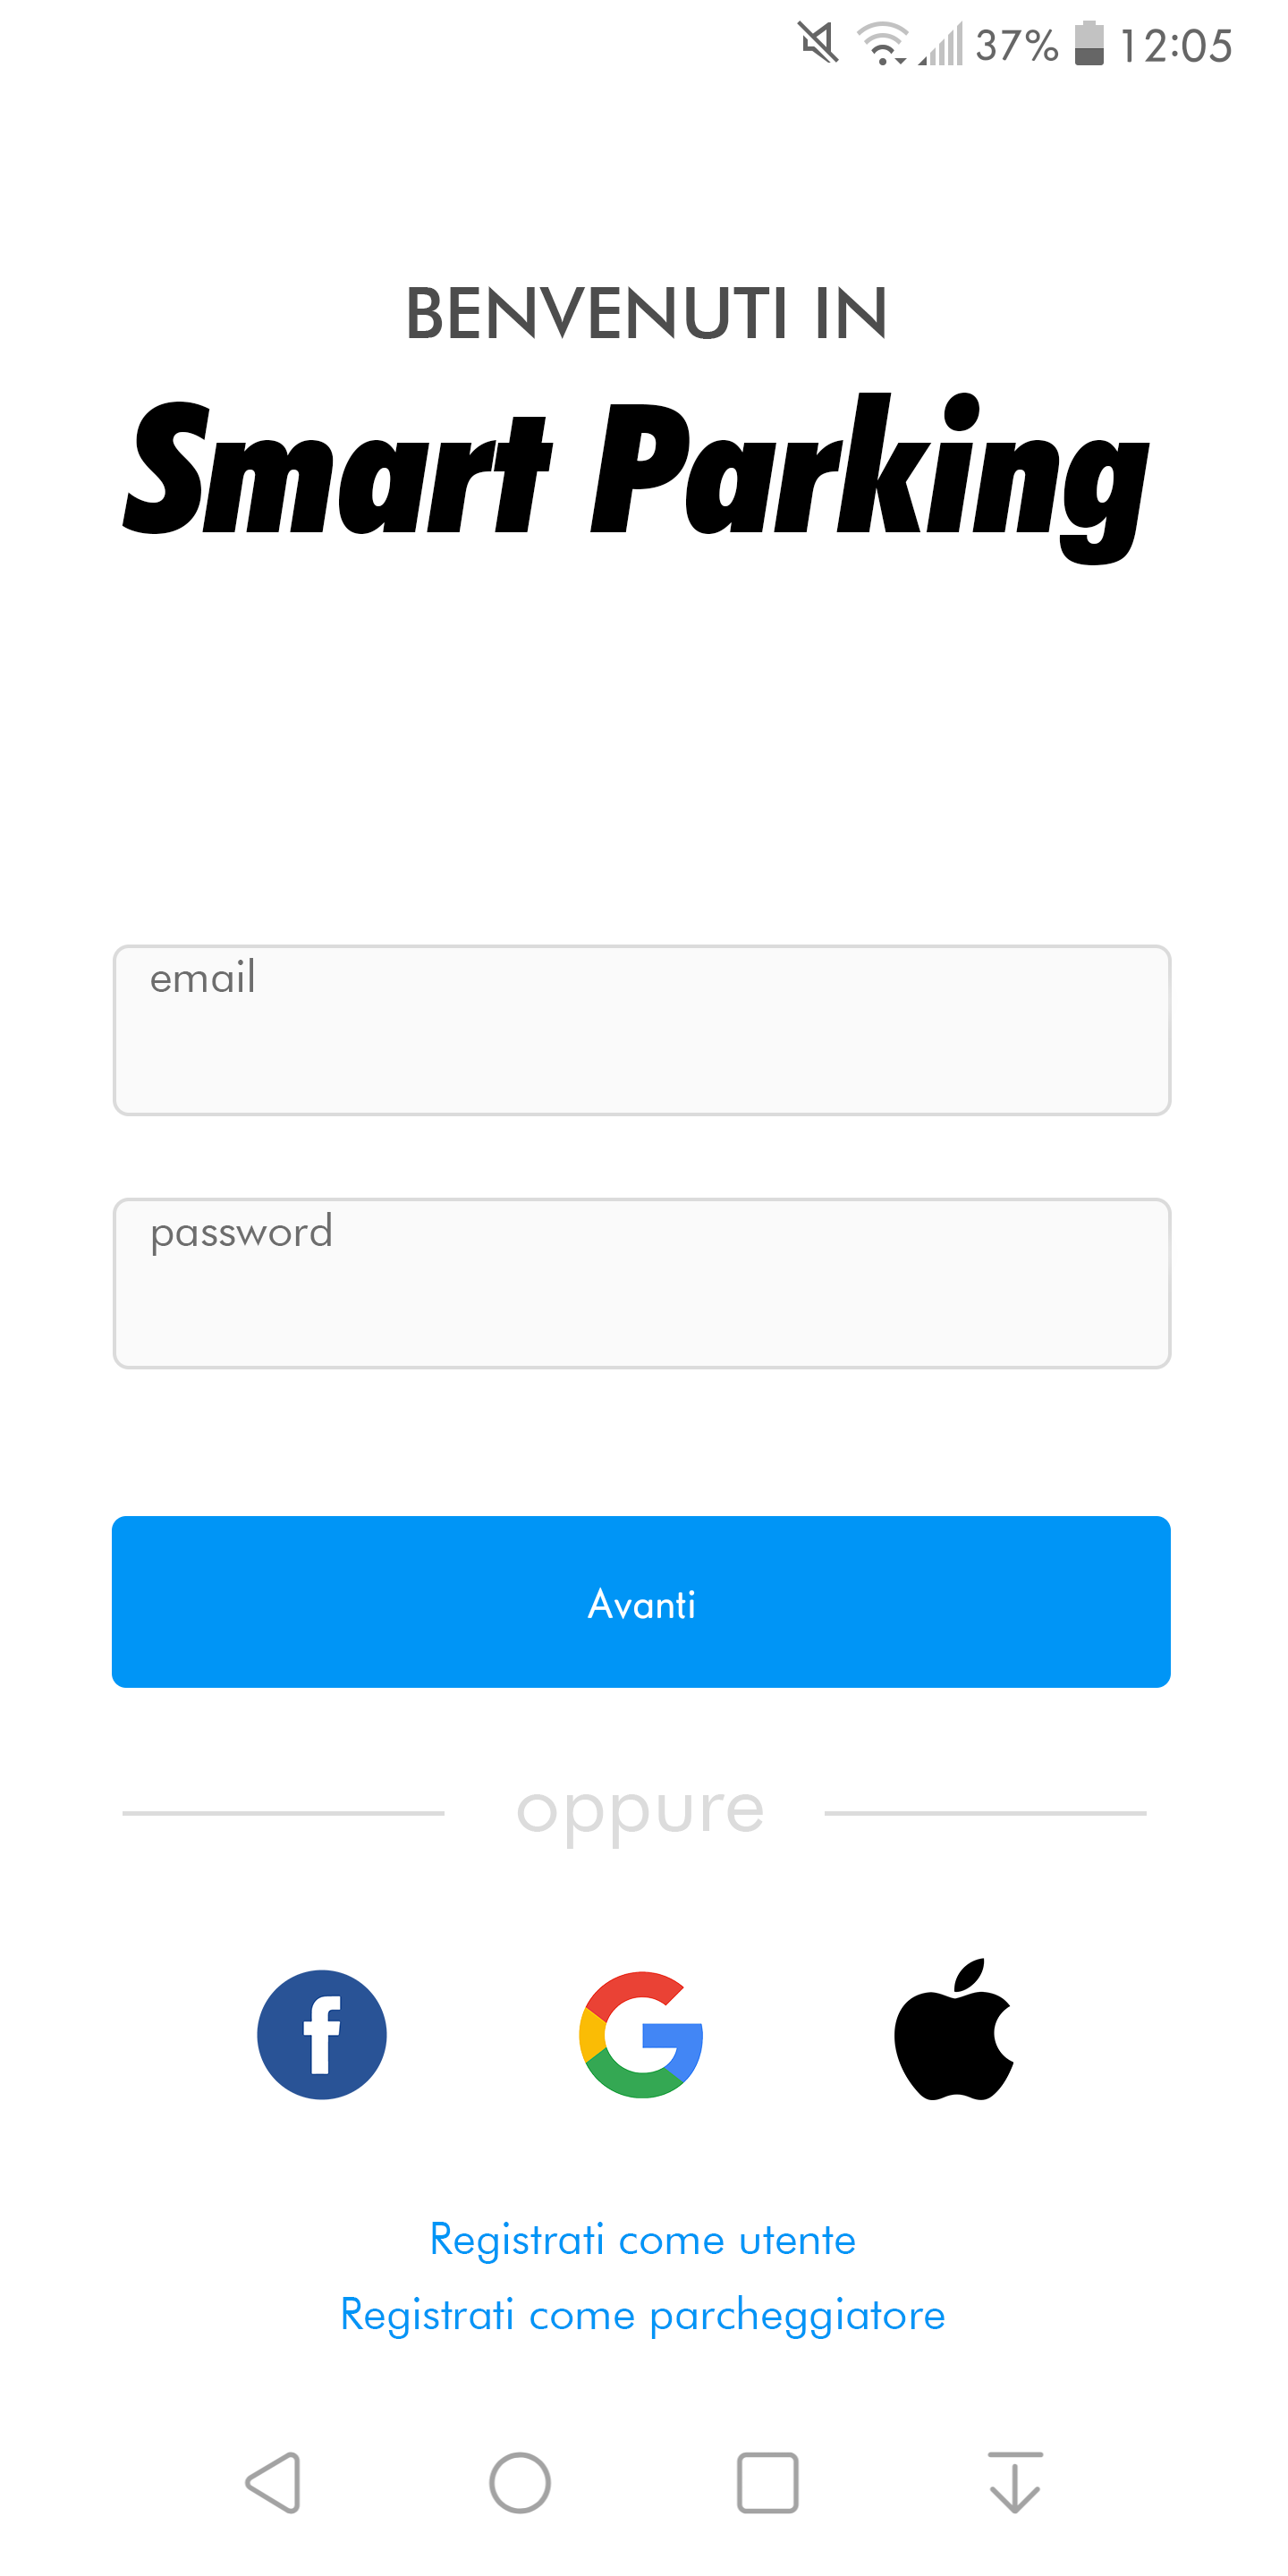
\includegraphics[scale=0.07,keepaspectratio, valign = c]{Img/primaSchermata.png}}}
        \\
    \end{tabular}
    \label{tab:login}
\end{table}
\begin{table}[H]
    \centering
    \begin{tabular}{m{0.4\linewidth} c c}
        Nel caso non si sia effettuato l'accesso con SSO, in queste due schermate vengono inseriti i dati dell'utente. All'invio dei dati, una mail di conferma viene inviata all'indirizzo email specificato contenente un link per confermare la mail, come descritto in \ref{itm:RF1} e secondo le limitazioni imposte in RNF9.1 e RNF9.2.
        &
        {\fbox{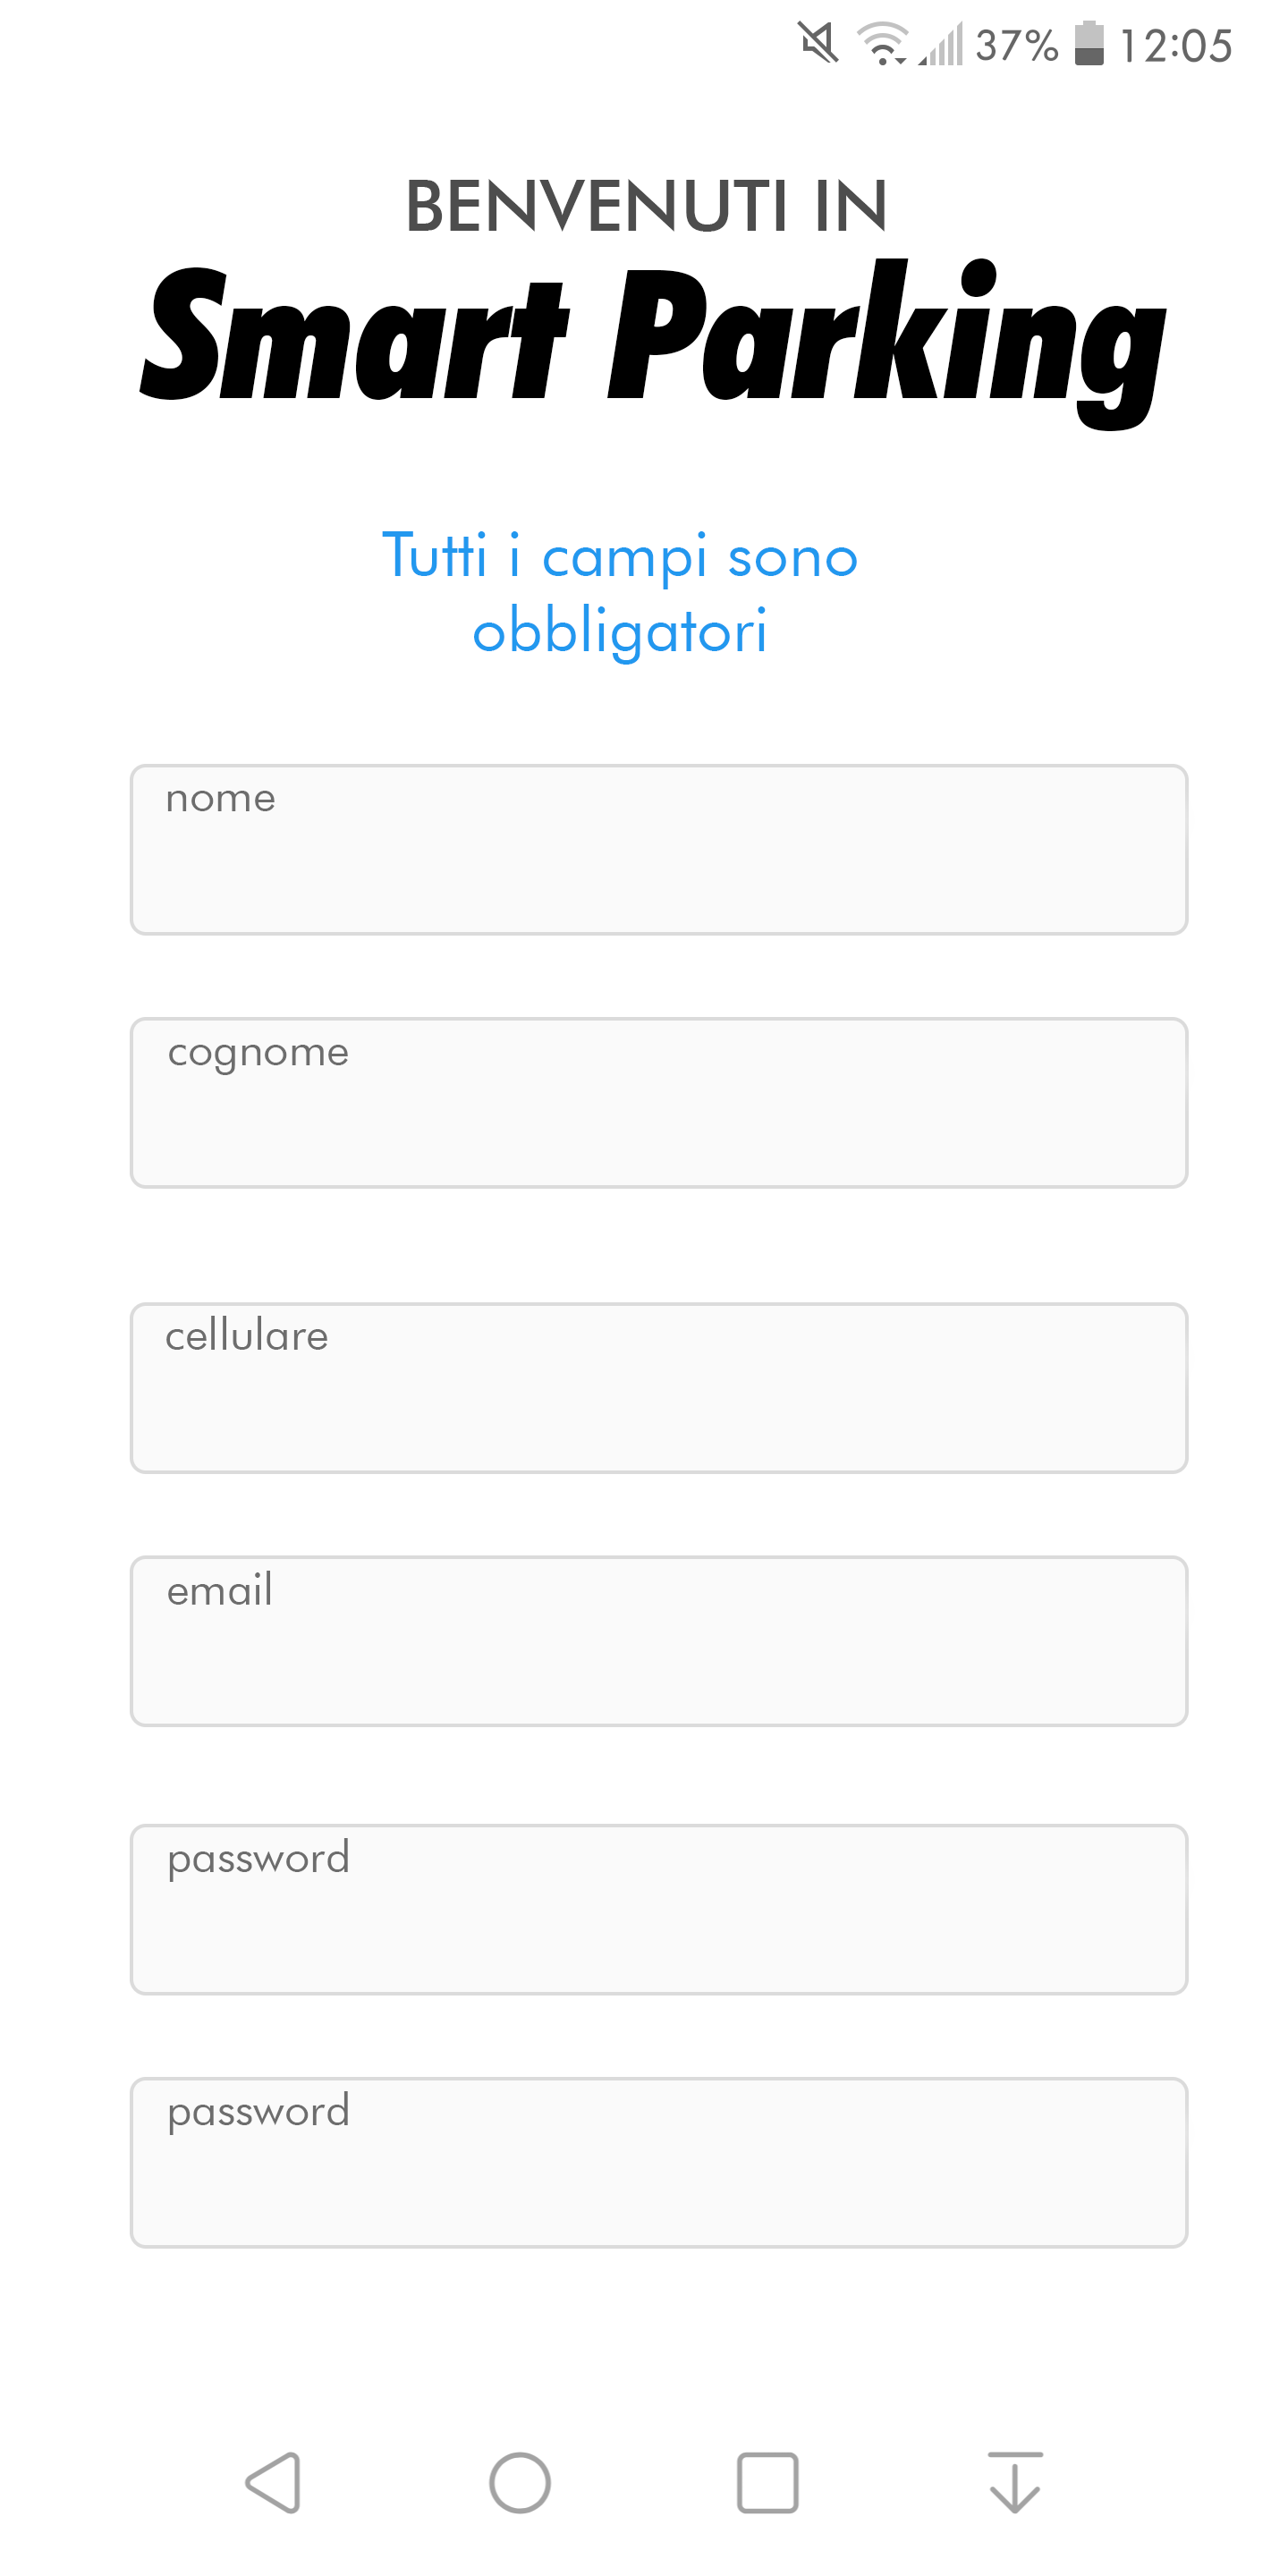
\includegraphics[scale=0.07,keepaspectratio, valign = c]{Img/registrazione1.png}}}
        &
        {\fbox{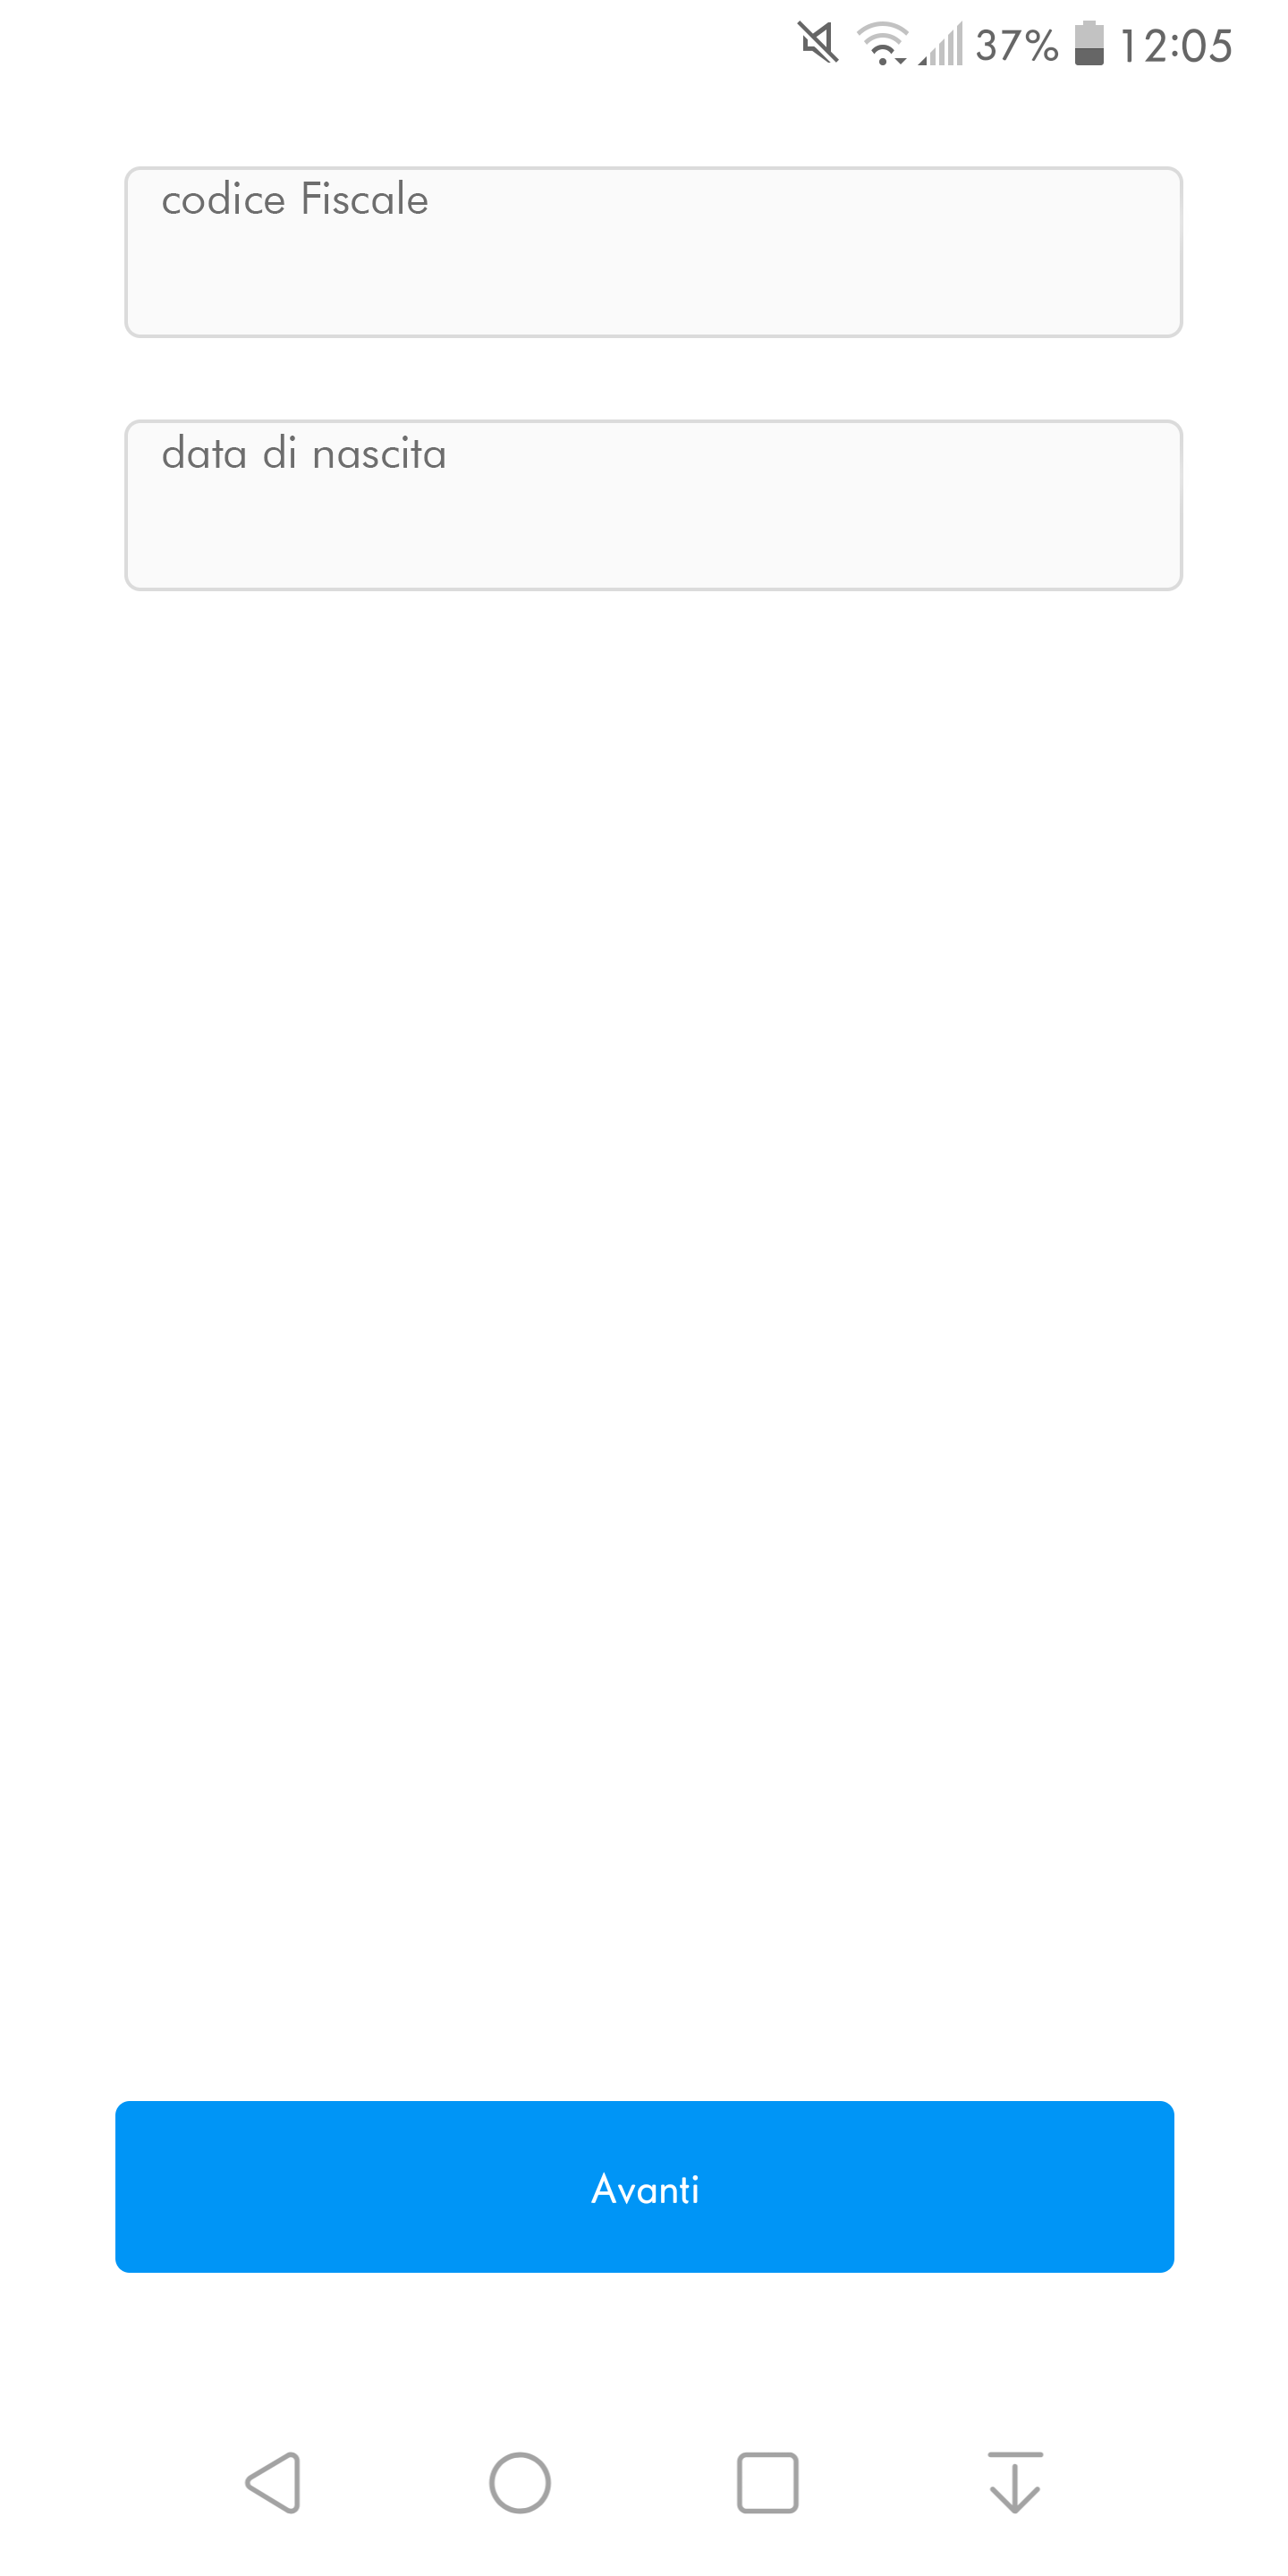
\includegraphics[scale=0.07,keepaspectratio, valign = c]{Img/registrazione2.png}}}
        \\
    \end{tabular}
    \label{tab:Registrazione}
\end{table}
\begin{table}[H]
    \centering
    \begin{tabular}{m{0.6\linewidth} c}
        Come spiegato in \ref{itm:RF4} In questa sezione l'utente autenticato inserisce le targhe delle macchine che vogliono utilizzare l'applicazione e le carte di credito utilizzate. Con il tasto "+" si può aggiungere un nuovo elemento. Entrambi i campi devono presentare almeno una componente secondo le limitazioni espresse in RNF9.3.
        &  
        {\fbox{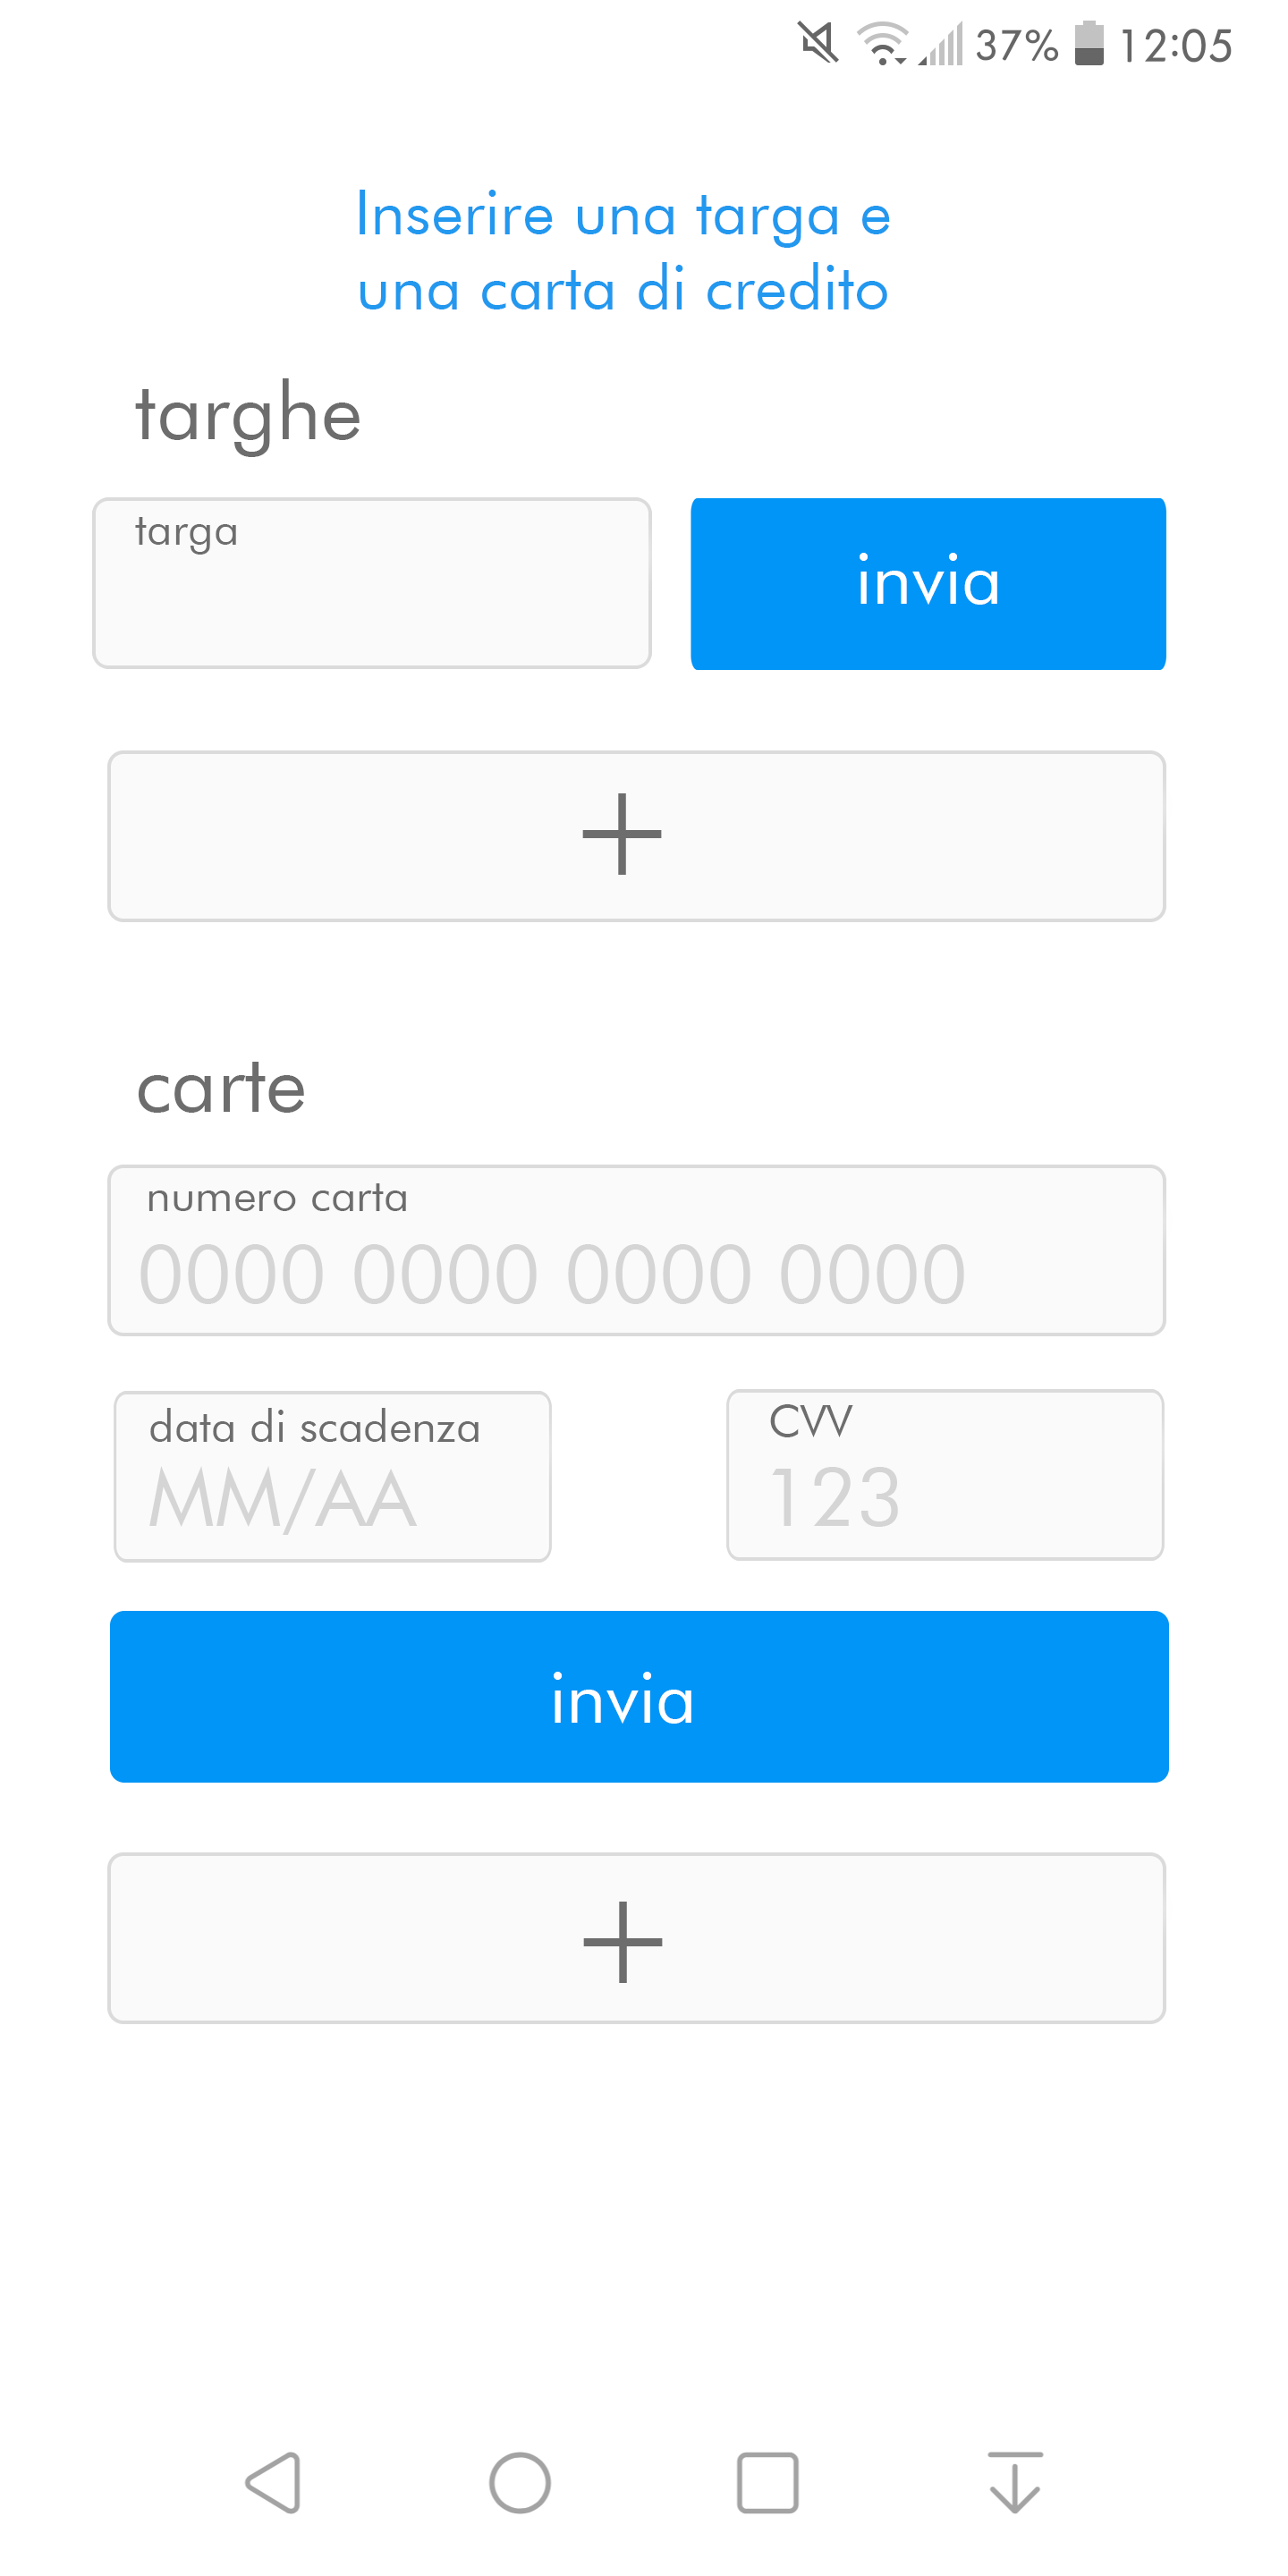
\includegraphics[scale=0.07,keepaspectratio, valign = c]{Img/cartaTargaPiu.png}}}
        \\
    \end{tabular}
    \label{tab:Targa&CC}
\end{table}
\begin{table}[H]
    \centering
    \begin{tabular}{m{0.6\linewidth} c}
        Attraverso il menù l'utente autenticato può navigare tra le schermate: "cerca parcheggio", "wallet", "prenotazioni", "possiedi un parcheggio?", "contattaci" e "logout". Inoltre, se l'utente autenticato è proprietario di uno o più parcheggi avrà a disposizione una voce nel menù ad hamburger che potrà utilizzare per gestire i suoi parcheggi.  \ref{itm:RF16}.
        &
        {\fbox{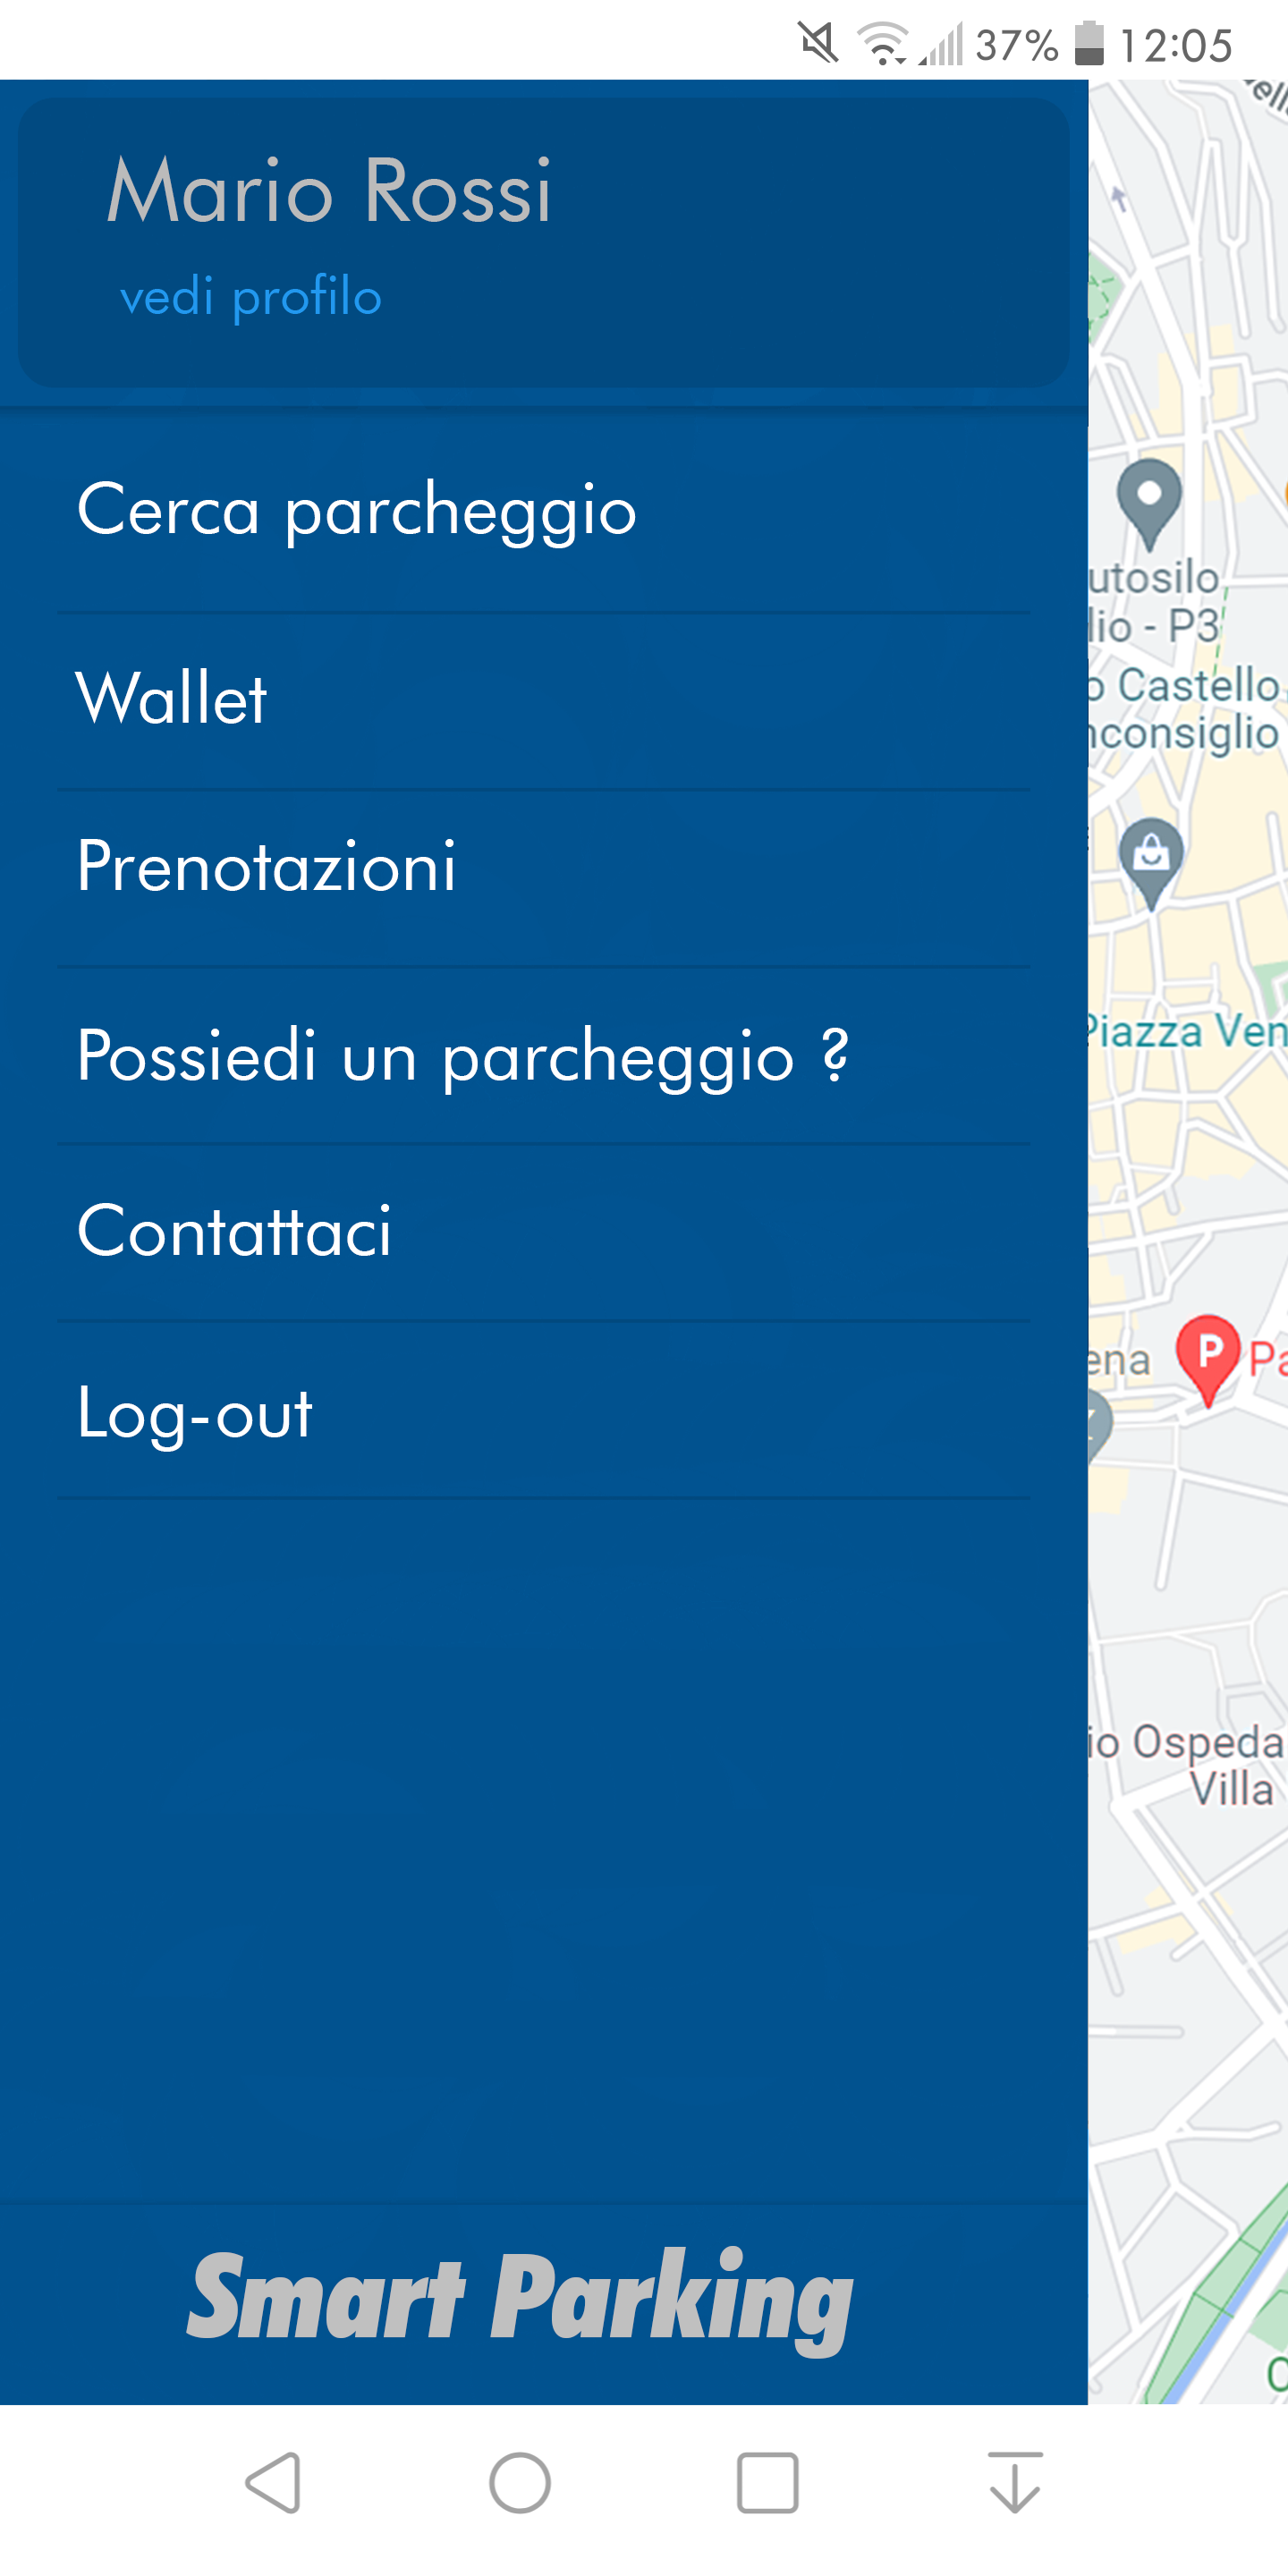
\includegraphics[scale=0.07,keepaspectratio, valign = c]{Img/menuHamburger.png}}}
        \\
    \end{tabular}
    \label{tab:Hamburger}
\end{table}
\begin{table}[H]
    \centering
    \begin{tabular}{m{0.6\linewidth} c}
        Una volta effettuato il login l'utente può interagire con google maps integrato nell'applicazione, che mostra la disponibilità dei parcheggi attraverso dei colori (verde, giallo e rosso). Selezionando la barra di ricerca l'utente può cercare un parcheggio secondo le indicazioni riportate nella figura di ricerca.
        & 
        {\fbox{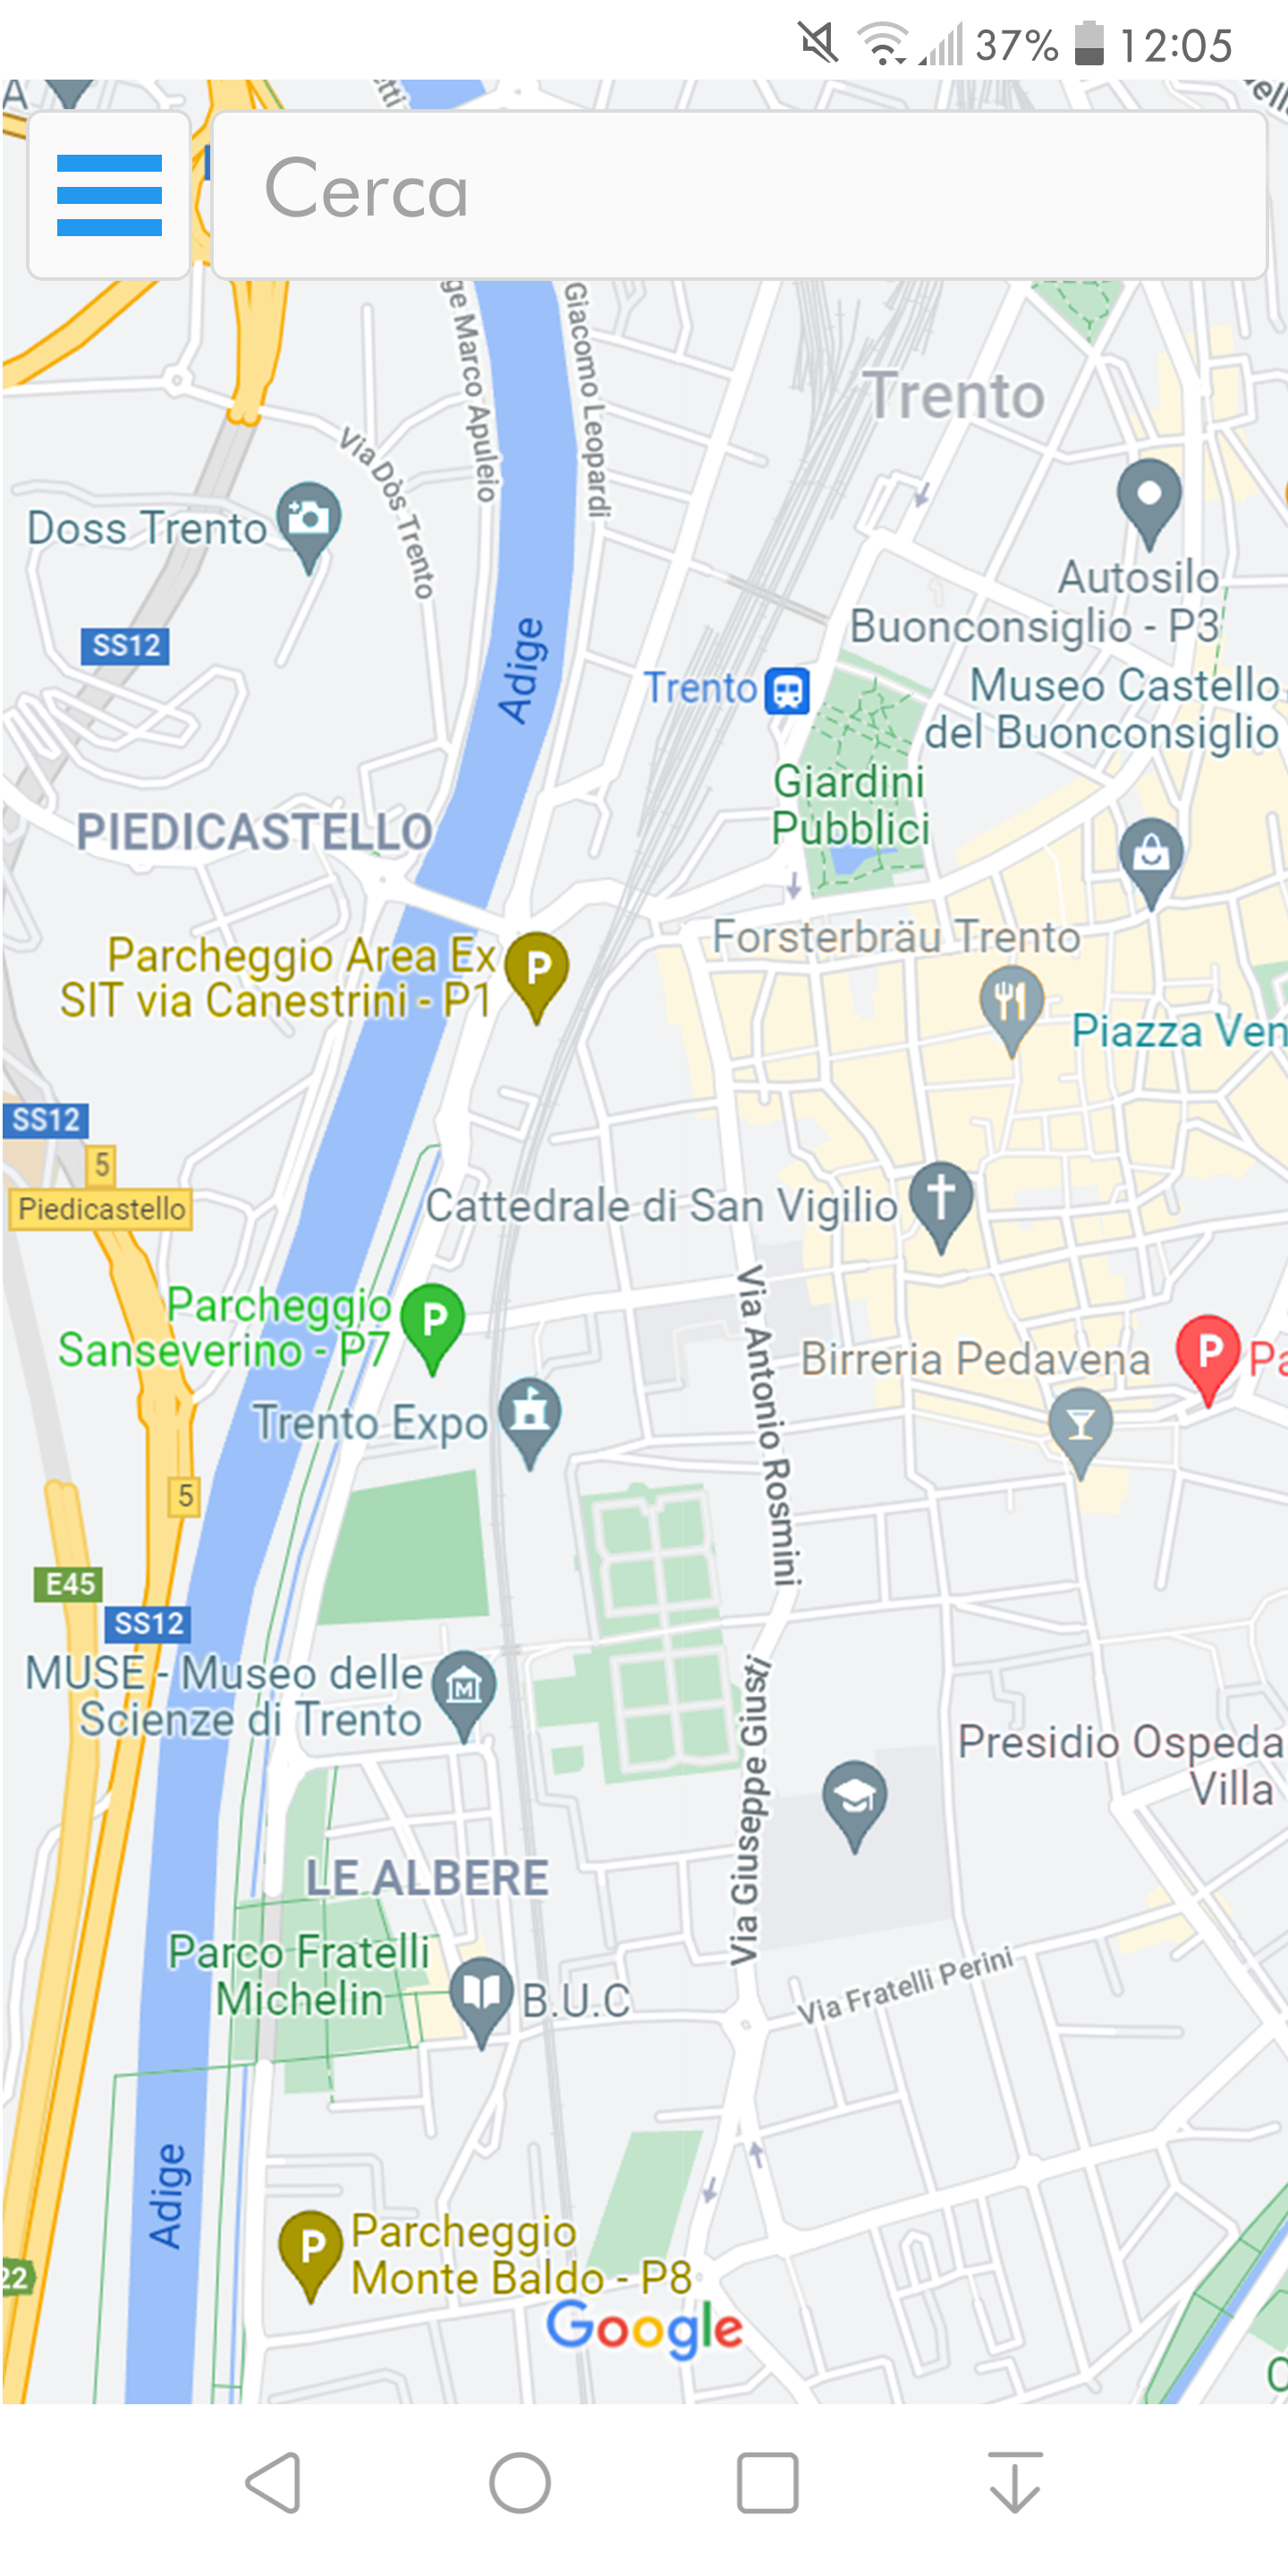
\includegraphics[scale=0.07,keepaspectratio, valign = c]{Img/home.png}}}
        \\ 
    \end{tabular}
    \label{tab:Home}
\end{table}

\begin{table}[H]
    \centering
    \begin{tabular}{m{0.6\linewidth} c}
        É possibile effettuare la ricerca applicando dei filtri in base a tariffa oraria e raggio. Il bottone "preferiti" apre la lista dei preferiti.
        &  
        {\fbox{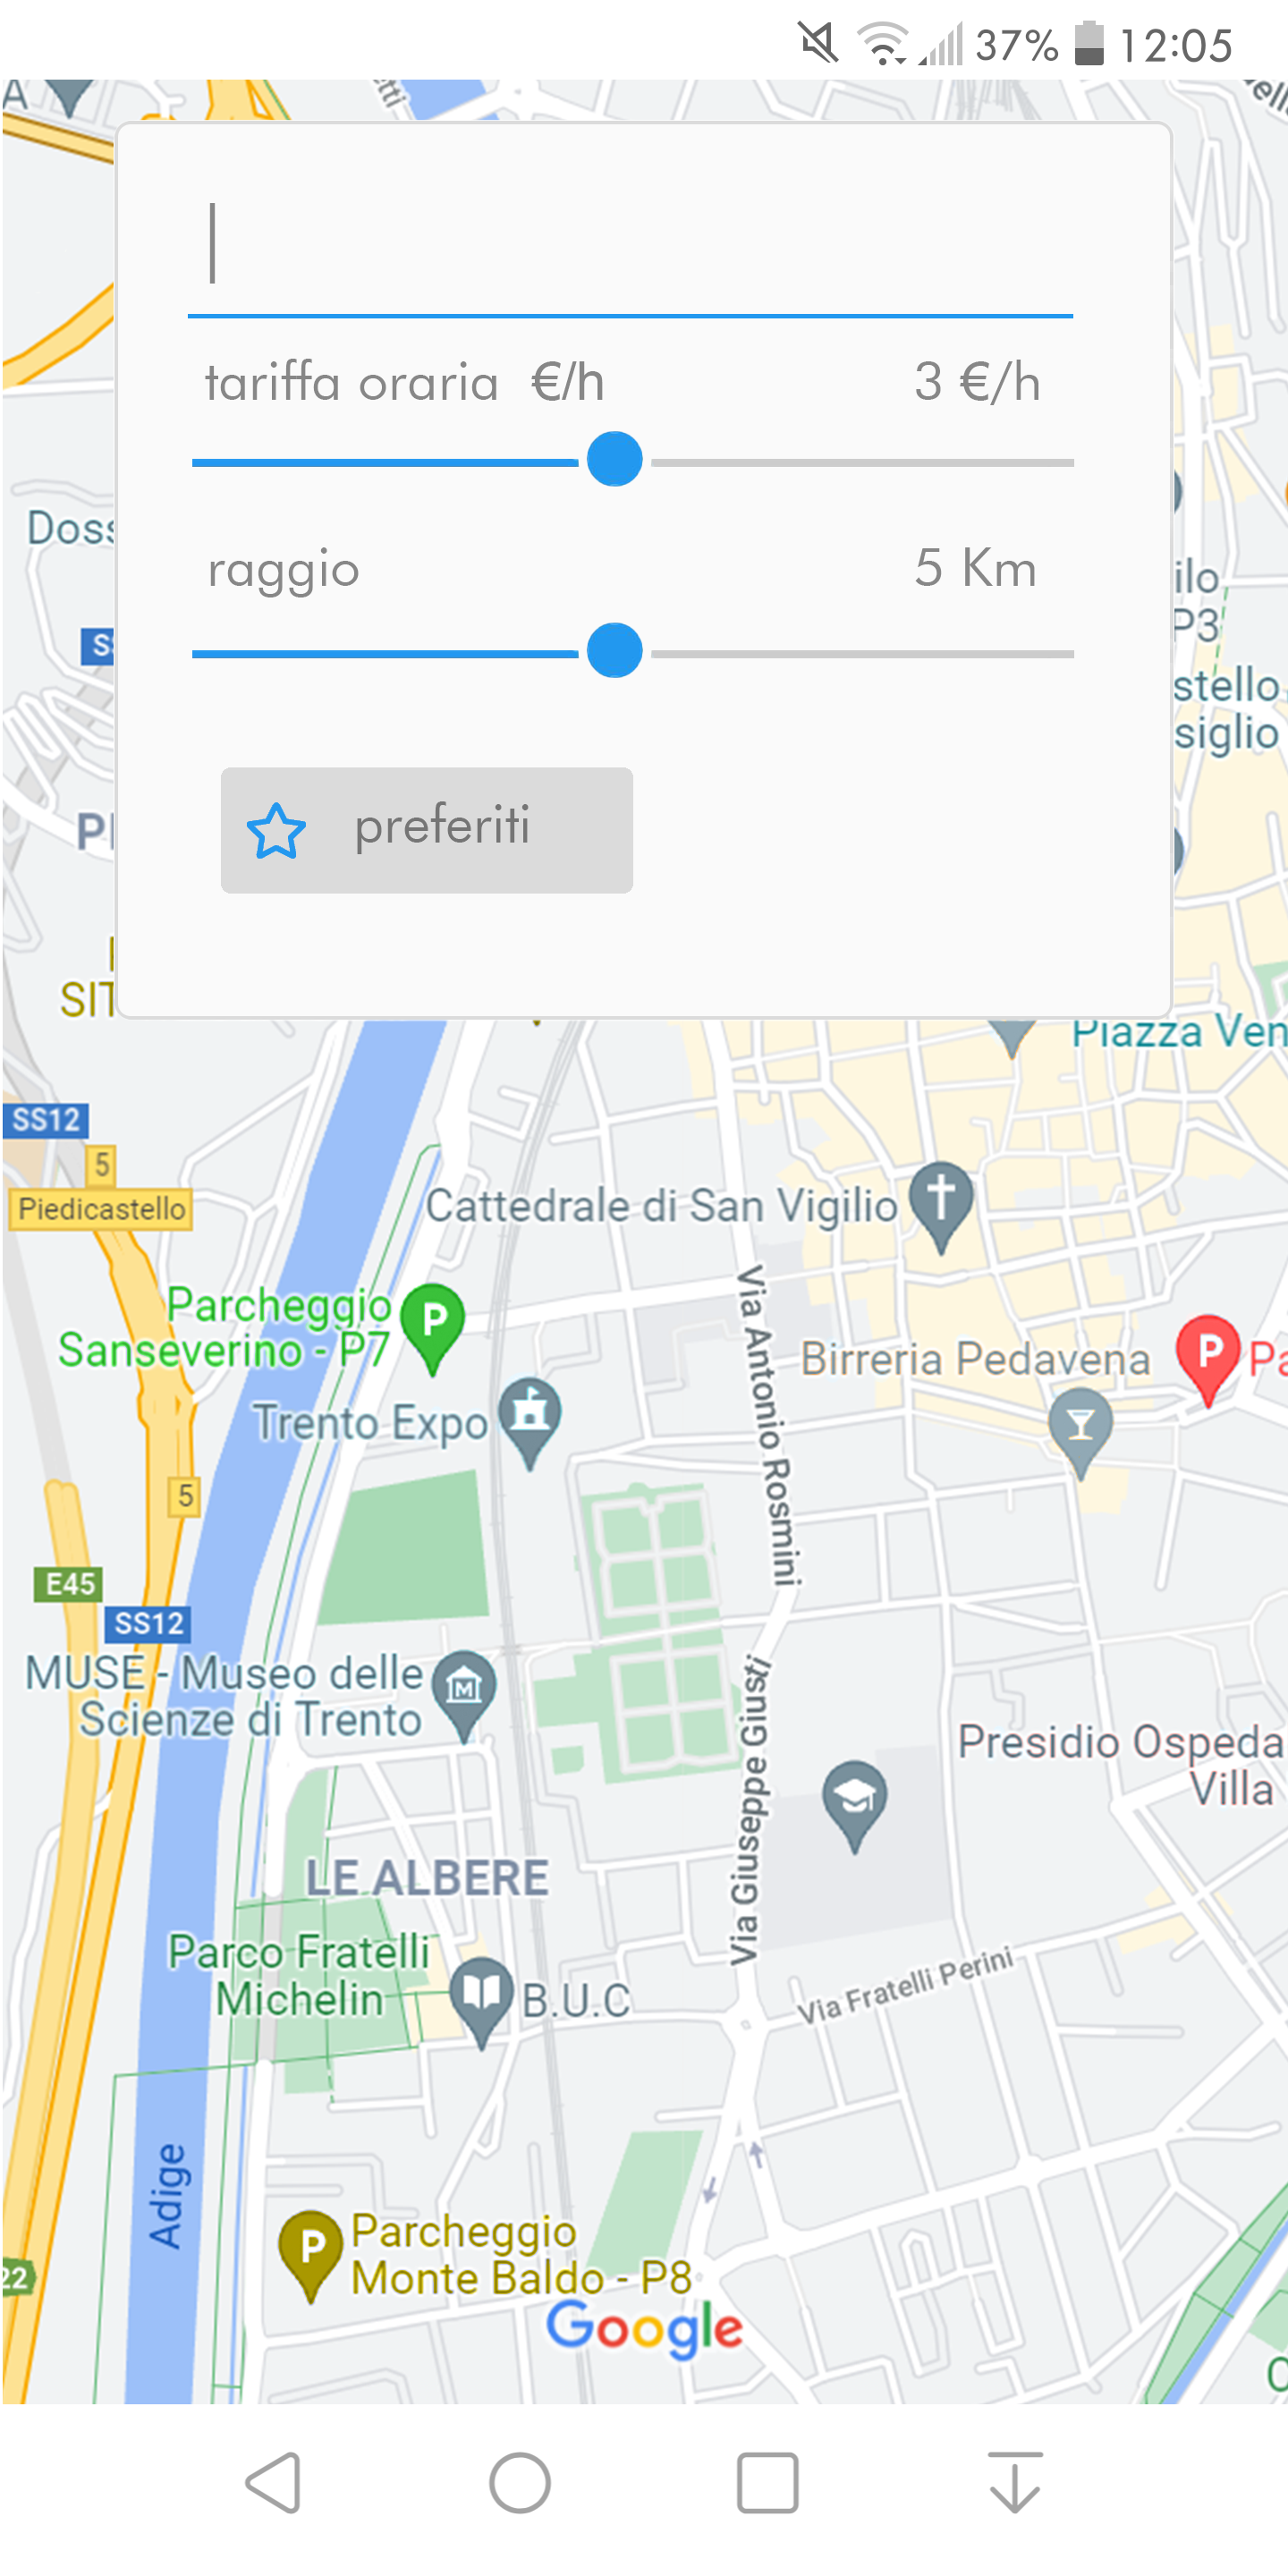
\includegraphics[scale=0.07,keepaspectratio, valign = c]{Img/ricerca.png}}} 
        \\
    \end{tabular}
    \label{tab:Ricerca}
\end{table}

\begin{table}[H]
    \centering
    \begin{tabular}{m{0.6\linewidth} c}
        Una volta effettuata la ricerca viene presentata una lista in base ai filtri applicati ed è possibile aggiungere o rimuovere i parcheggi ai preferiti. Il bottone "ordina" apre un filtro, come visto in \ref{itm:RF8}.
         &  
        {\fbox{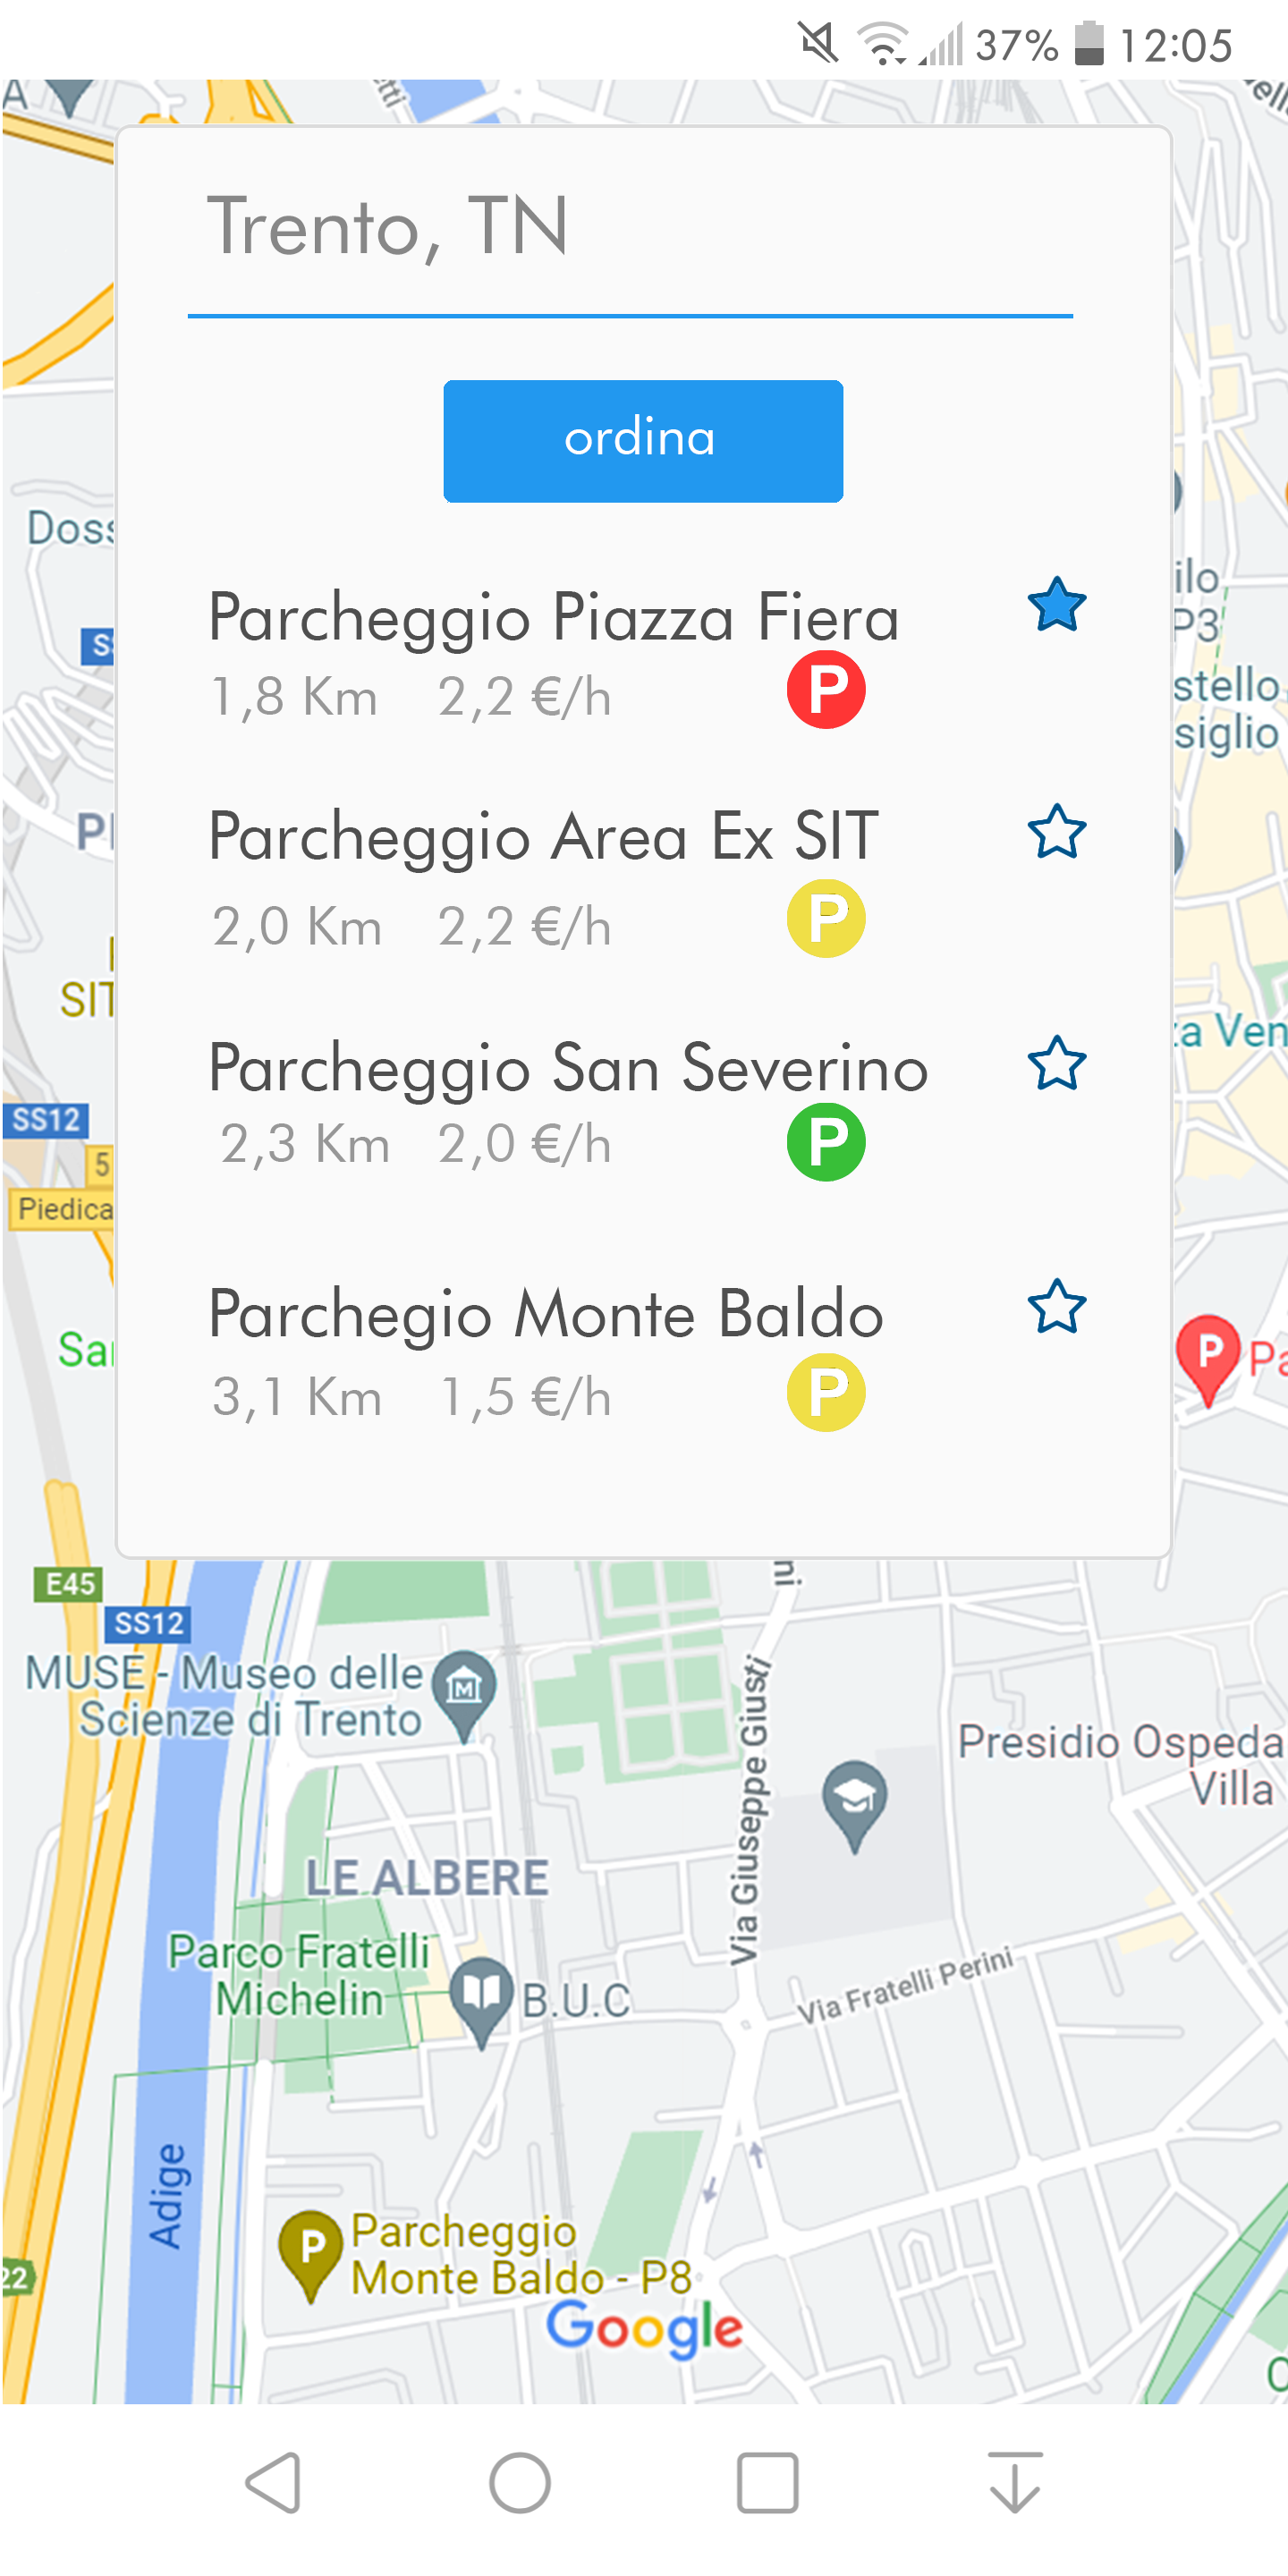
\includegraphics[scale=0.07,keepaspectratio, valign = c]{Img/ricercaFatta.png}}}
         \\
         & 
    \end{tabular}
    \label{tab:RicercaFatta}
\end{table}

\begin{table}[H]
    \centering
    \begin{tabular}{m{0.6\linewidth} c}
        Una volta selezionato un parcheggio dalla finestra precedente è possibile selezionare il tempo di sosta mediante uno slider e confermare con il tasto "prenota".
        \textcolor{red}{Se lo slider viene portato ad una durata maggiore di 24h la finestra di prenotazione si allarga includendo delle sezioni dove poter selezionare il giorno e la fascia oraria della prenotazione}. La gestione delle prenotazioni da parte del sistema è descritta in \ref{itm:RF20} e l'accettazione delle suddette è descritto secondo il \ref{itm:RF23}.
        &  
        {\fbox{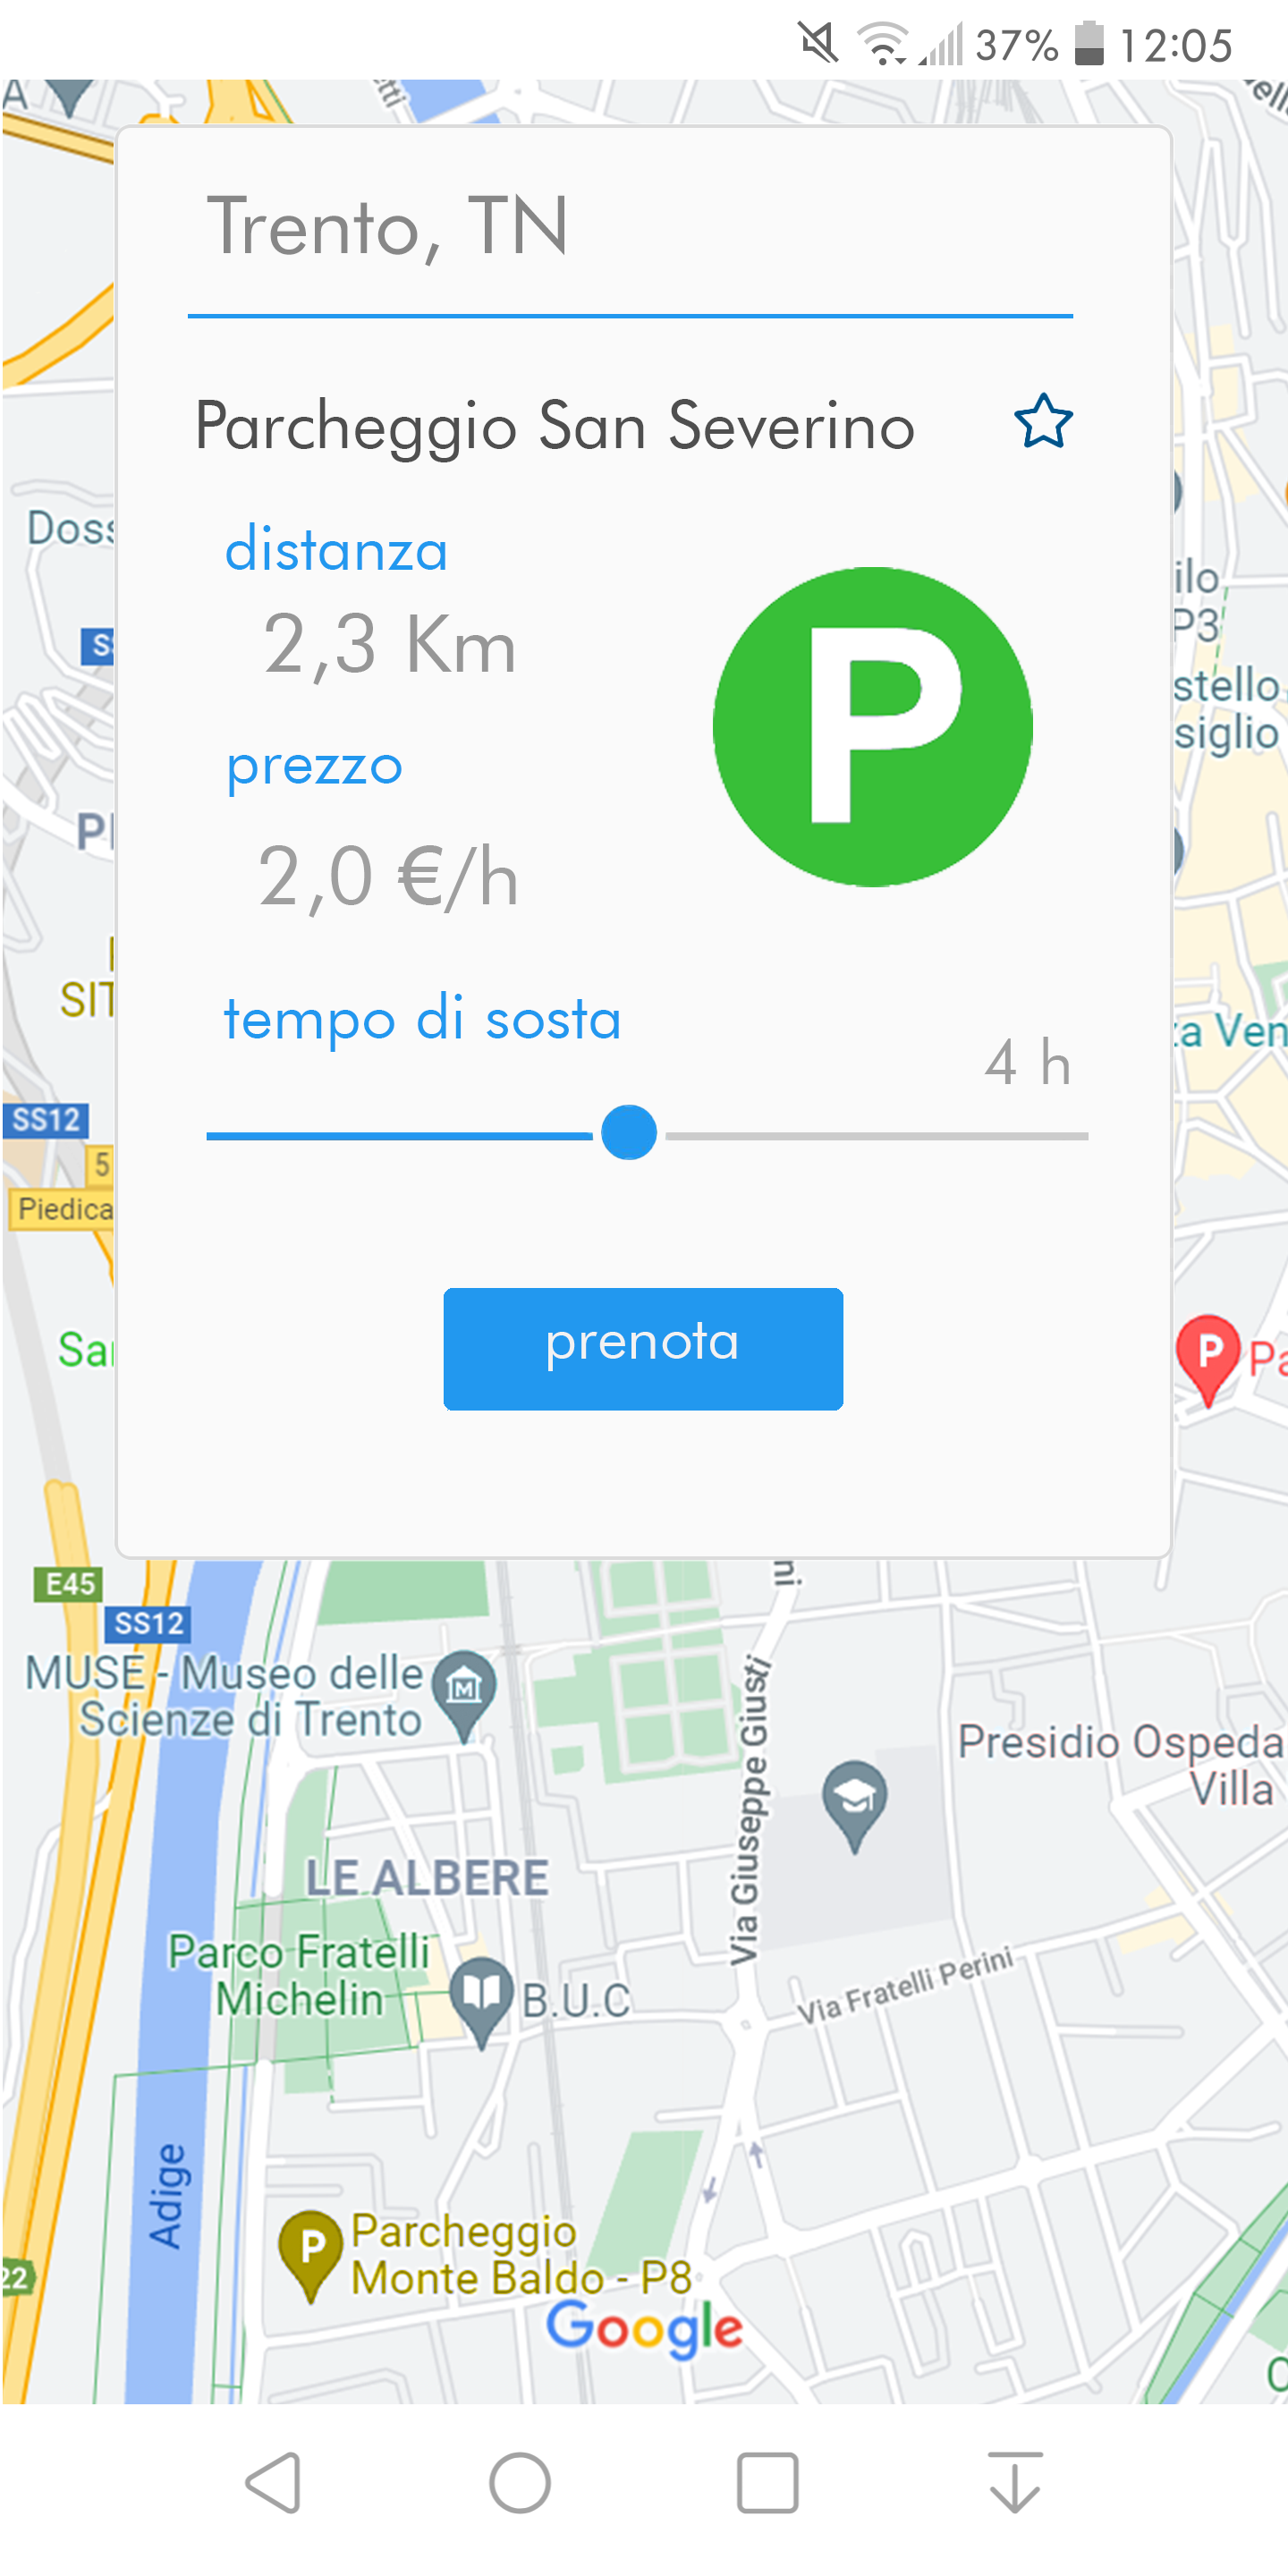
\includegraphics[scale=0.07,keepaspectratio, valign = c]{Img/prenotazione.png}}}
        \\
    \end{tabular}
    \label{tab:prenotazione}
\end{table}

\begin{table}[H]
    \centering
    \begin{tabular}{m{0.6\linewidth} c}
        In questa schermata l'utente può visionare lo stato del wallet (saldo e transazioni) ed effettuarne la ricarica tramite una carta di credito memorizzata nell'account. 
        &
        {\fbox{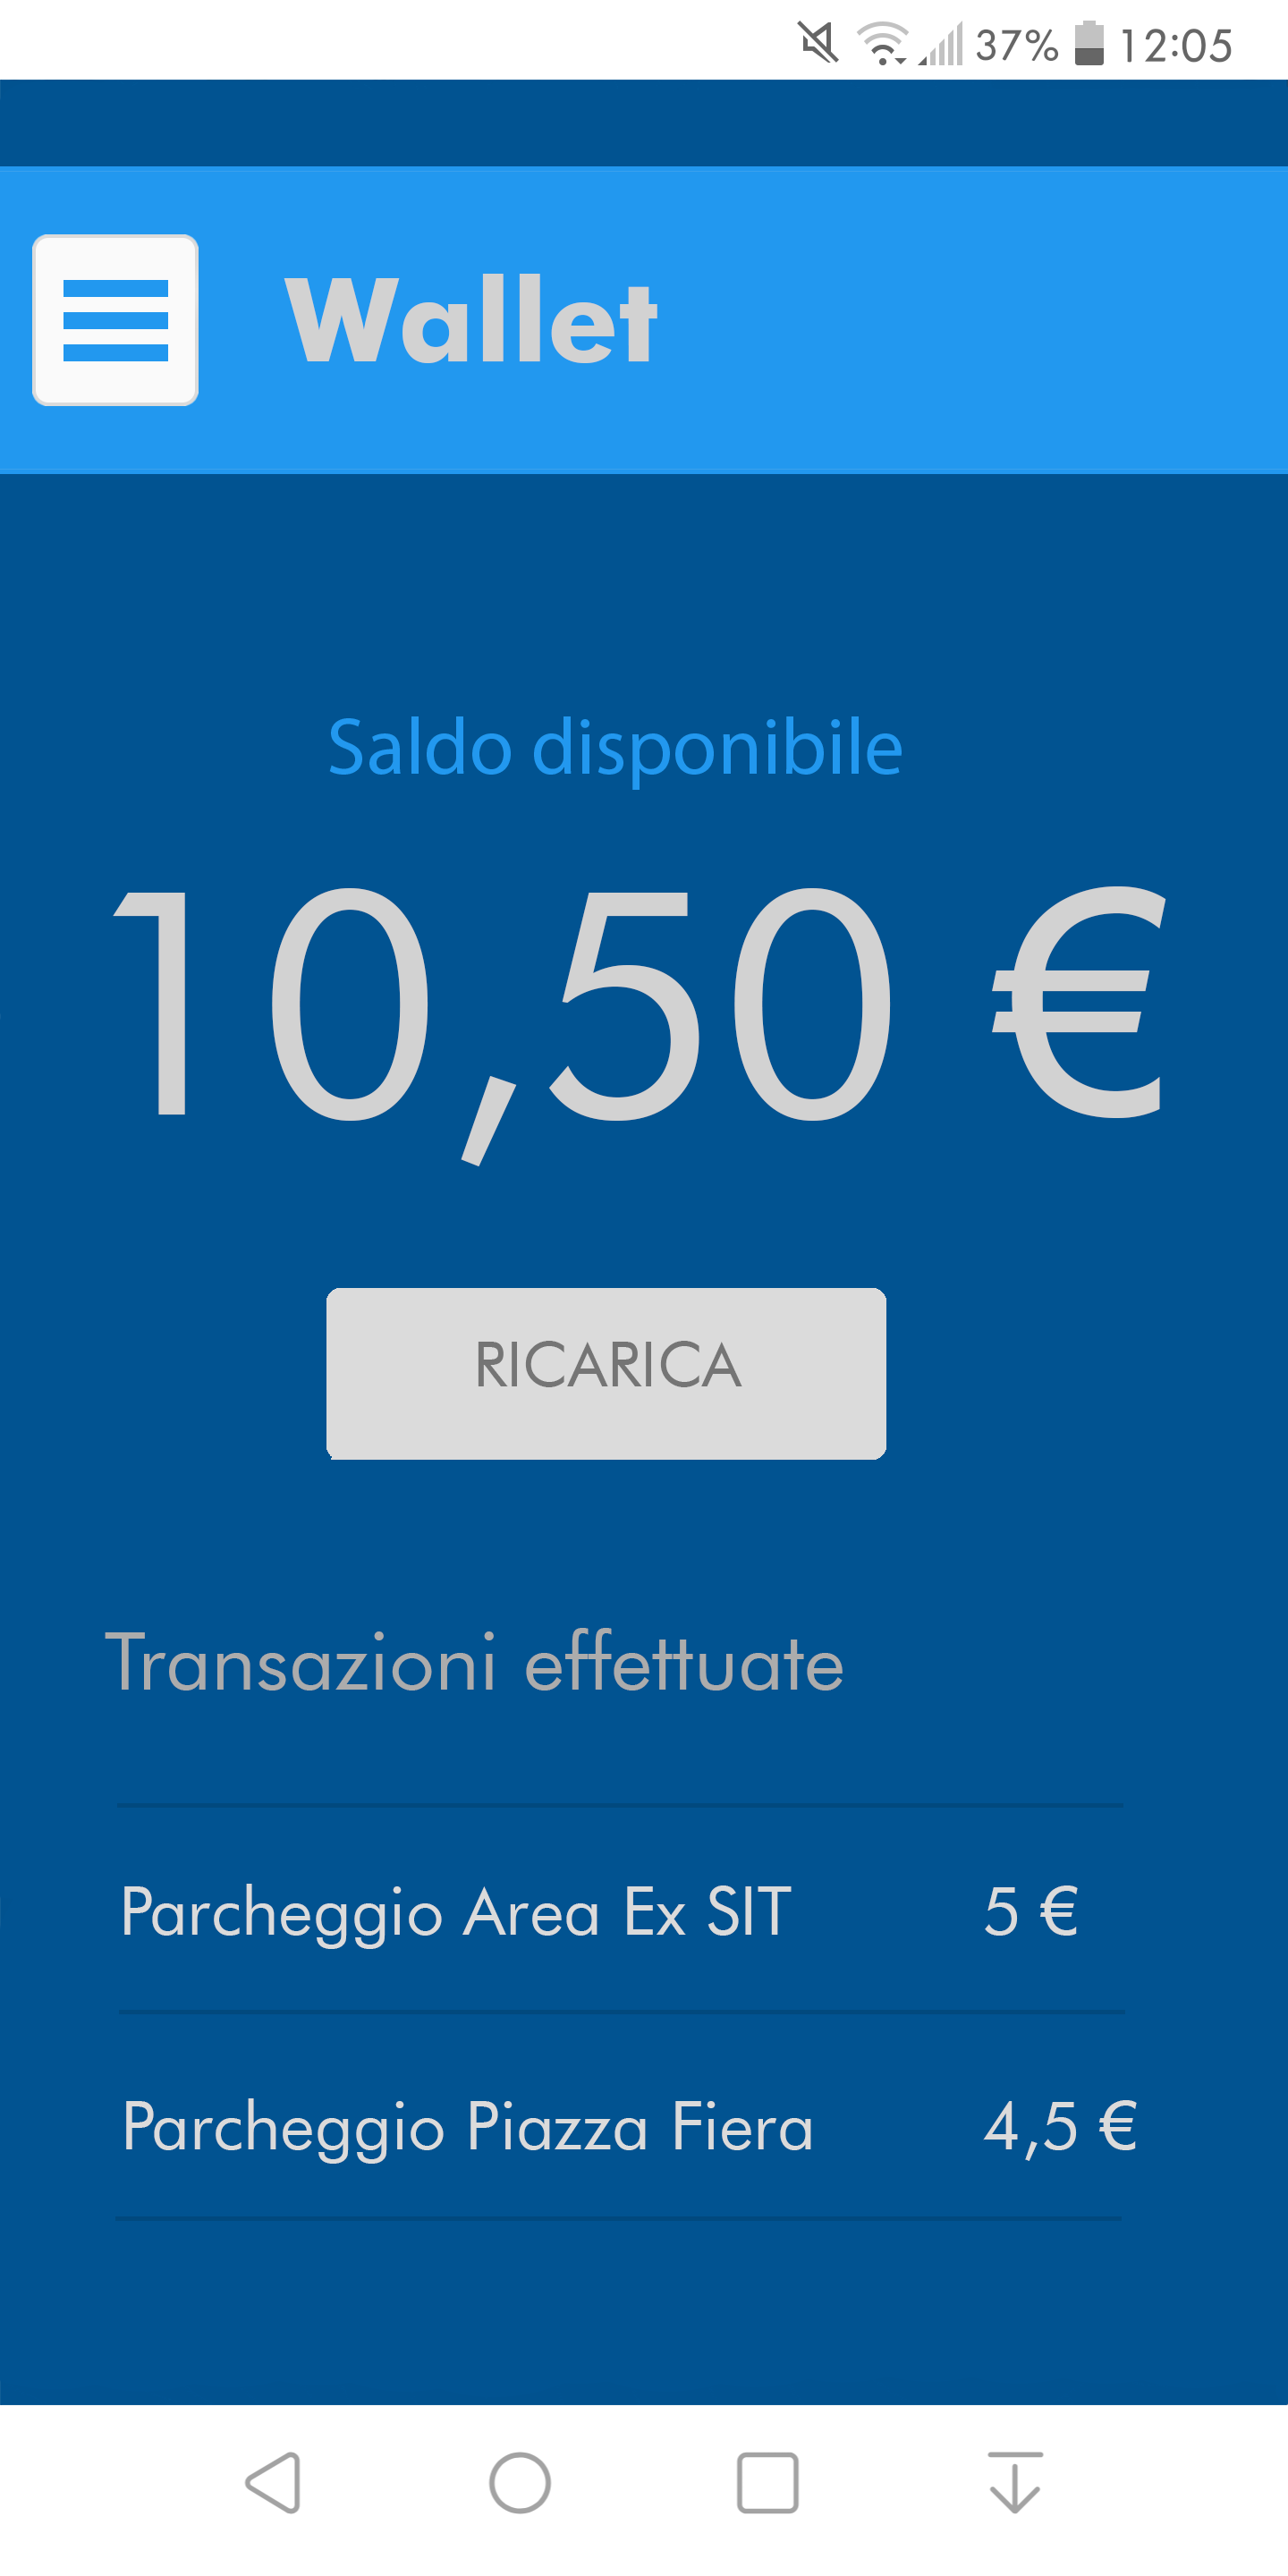
\includegraphics[scale=0.07,keepaspectratio, valign = c]{Img/wallet.png}}}
        \\
         & 
    \end{tabular}
    \label{tab:wallet}
\end{table}

\begin{table}[H]
    \centering
    \begin{tabular}{m{0.6\linewidth} c}
        Da questa sezione è possibile accedere alla lista delle prenotazioni effettuate. Il bottone con il cestino serve a cancellare una prenotazione, seguendo le indicazioni fornite in \ref{itm:RF21}.
        & 
        {\fbox{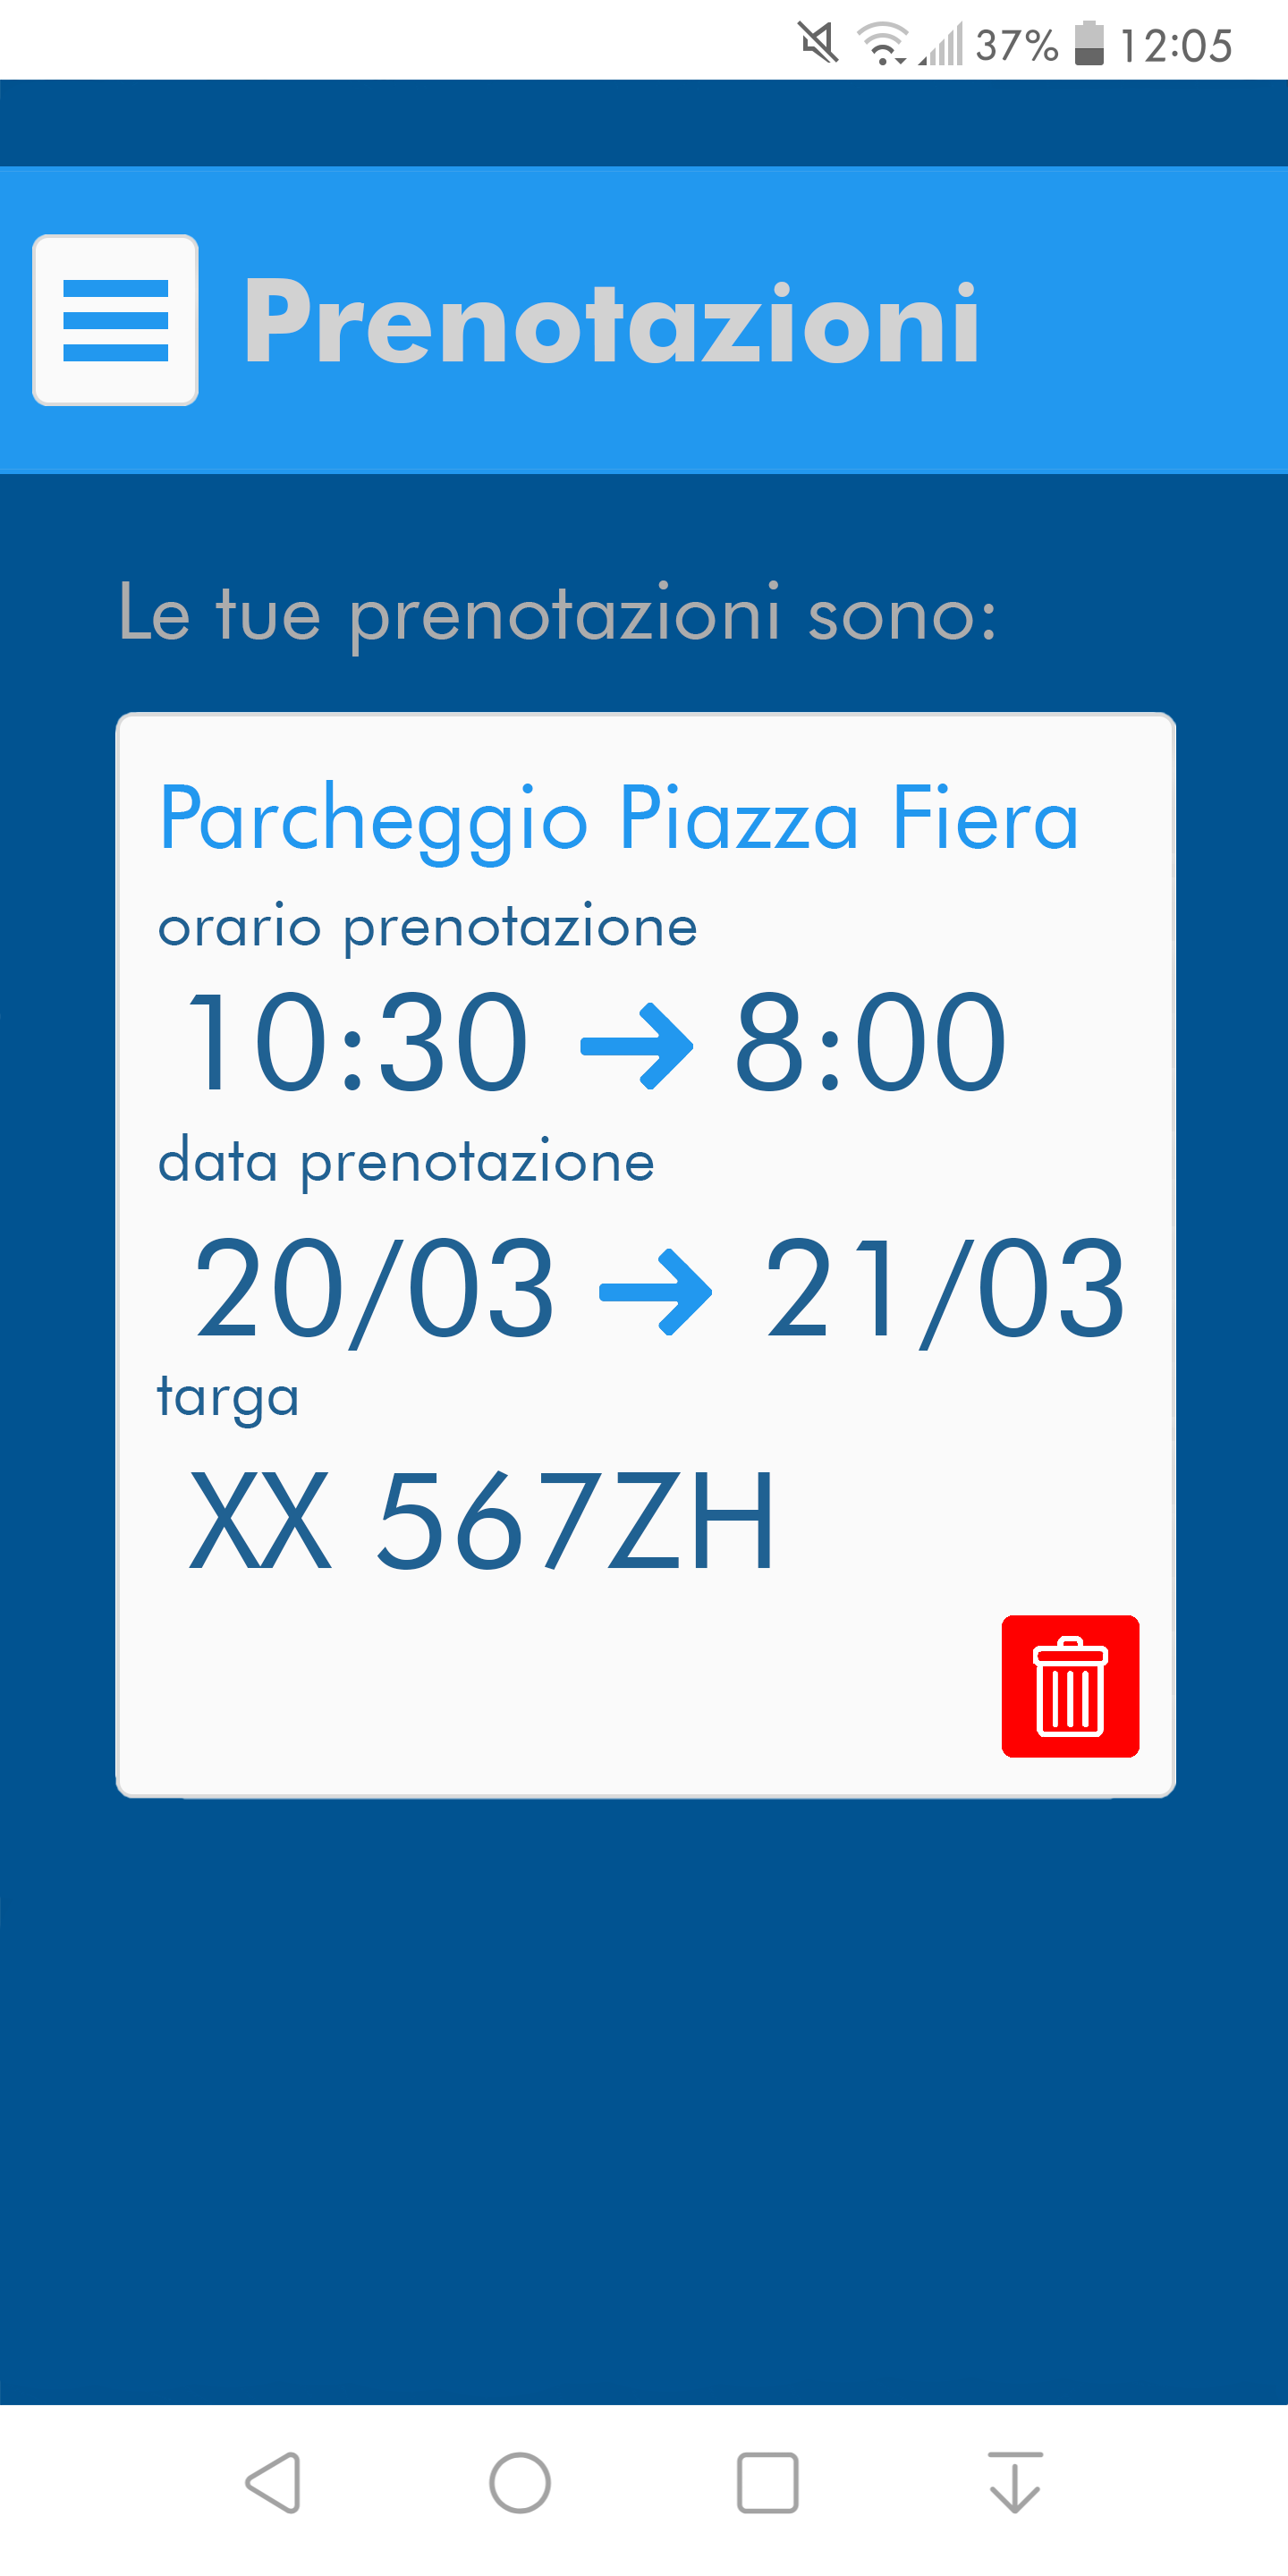
\includegraphics[scale=0.07,keepaspectratio, valign = c]{Img/listaPrenotazioni.png}}}
        \\
    \end{tabular}
    \label{tab:listaPrenotazioni}
\end{table}

\begin{table}[H]
    \centering
    \begin{tabular}{m{0.6\linewidth} c}
        Si può accedere in questa sezione selezionando "vedi profilo" dal menù ad hamburger. Qui l'utente può visualizzare i suoi dati e premendo il tasto "MODIFICA" può modificare la password come visto in RNF9.2, l'indirizzo email (la mail verrà verificata come alla prima registrazione vista nel punto) \ref{itm:RF2}.
        &  
        {\fbox{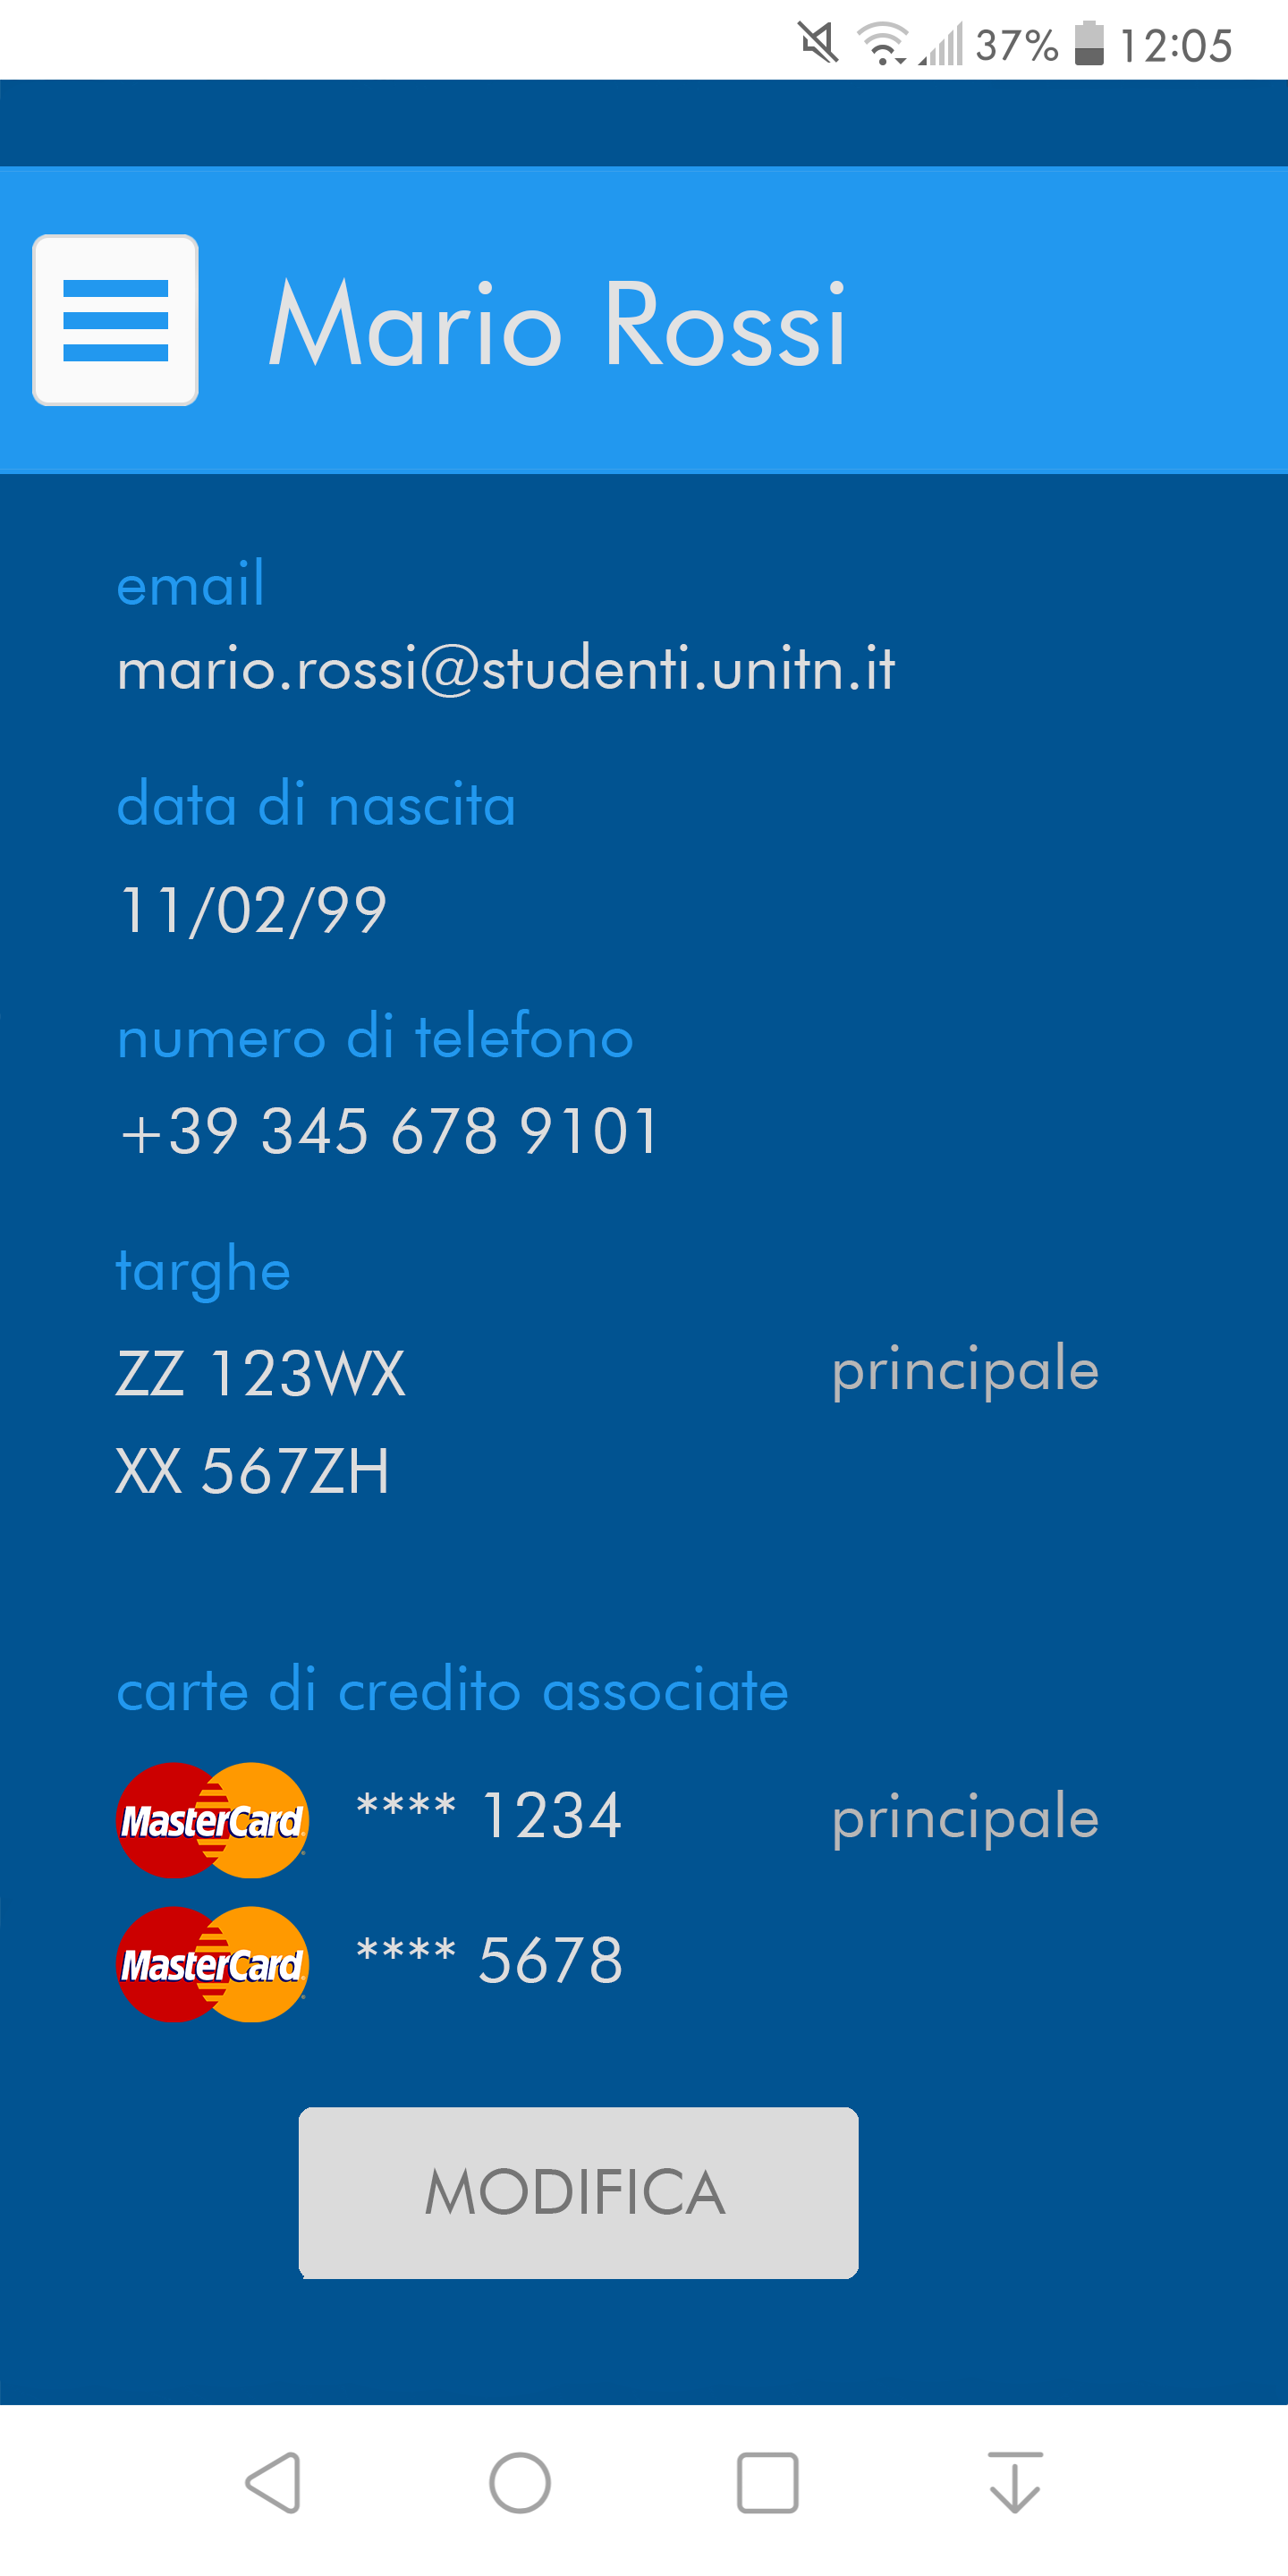
\includegraphics[scale=0.07,keepaspectratio, valign = c]{Img/datiPersonali.png}}}
        \\
    \end{tabular}
    \label{tab:my_label}
\end{table}

\begin{table}[H]
    \centering
    \begin{tabular}{m{0.6\linewidth} c}
        Questa sezione appare nel menù ad hamburger solo nel caso l'utente sia proprietario di un parcheggio. In questa sezione l'utente può modificare i dati del parcheggio e con il tasto "+" può aggiungere un parcheggio, nel caso ne possieda più di uno.
        & 
        {\fbox{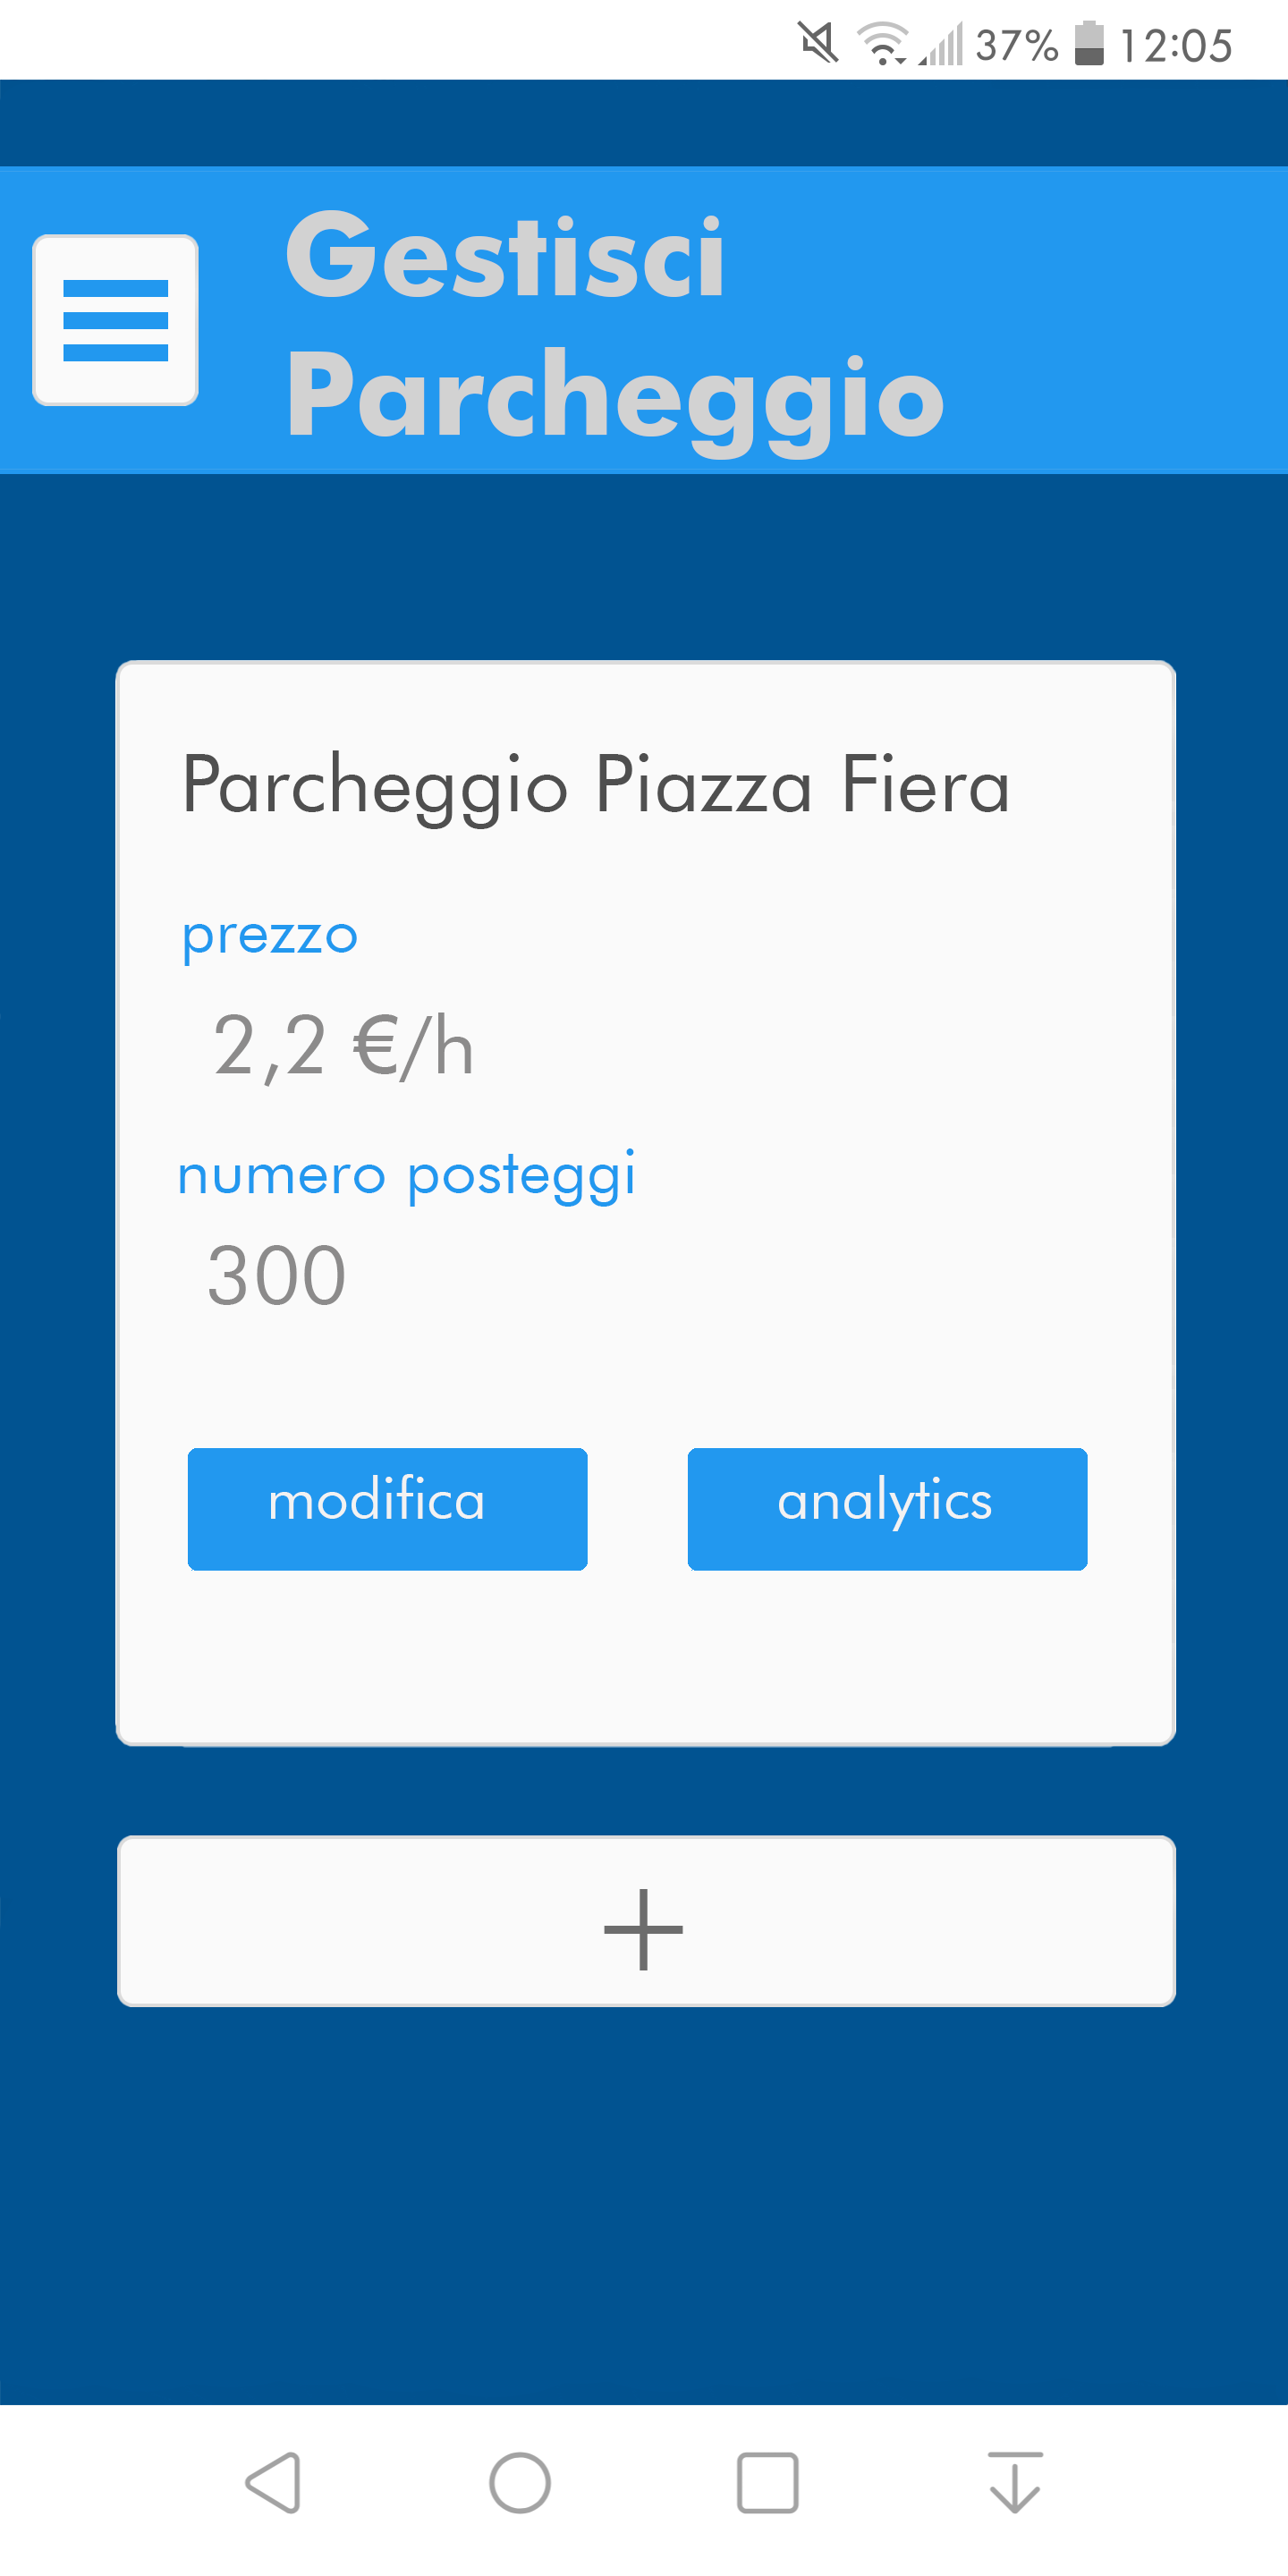
\includegraphics[scale=0.07,keepaspectratio, valign = c]{Img/gestisciParcheggio.png}}}
        \\
    \end{tabular}
    \label{tab:gestisciParcheggio}
\end{table}

\pagebreak
Alcune schermate del menù ad hamburger sono state omesse perché facilmente implementabili e con somiglianza ad altre rappresentate sopra:
\begin{itemize}
    \item "possiedi un parcheggio?" porta ad una finestra di registrazione simile all'immagine , inserendo nome del parcheggio, posti disponibili, città, via, CAP, tariffa oraria e orari di apertura del parcheggio. Alla fine della compilazione del form viene richiesto di caricare un file pdf/immagine che attesta la proprietà dell'immobile.
    \item "Contattaci" porta ad una schermata contenente una sezione in cui si descrive il problema o la domanda ed in basso un bottone con scritto "INVIA" che invia il form ad una mail di un centro assistenza.
    \item "Log Out" permette all'utente di effettuare il log out dall'applicazione. In questo caso al prossimo avvio verrà riportato alla schermata di accesso.
\end{itemize}
\section{Back End}
\textbf{Google Maps}
\begin{itemize}
    \item La nostra applicazione implementa \textbf{Google Maps} in quando ci permette di utilizzare le loro mappe che sono sempre in aggiornamento. Inoltre, possiamo mostrare i parcheggi disponibili ed utilizzare la sua funzione di navigazione per fornire il miglior percorso per raggiungere il parcheggio selezionato.
\end{itemize}
\textbf{Autenticazione Google - Apple - Facebook}
\begin{itemize}
    \item Permettiamo ai nostri utenti di effettuare il login attraverso google, facebook ed apple perchè sono un’\textbf{alternativa sicura} per effettuare il login nella nostra applicazione.  
\end{itemize}
\textbf{Videocamera - Sbarre del parcheggio}
\begin{itemize}
    \item La \textbf{videocamera} del parcheggio viene utilizzata per riconoscere le targhe delle macchine che accedono al parcheggio dopo aver prenotato un posto attraverso la nostra applicazione. Così facendo l’accesso può essere effettuato dall’utente facendo alzare le sbarre del parcheggio \textbf{senza dover prendere il biglietto} e registrare l’accesso nel sistema del parcheggio.
\end{itemize}
\textbf{Localizzazione GPS del telefono}
\begin{itemize}
    \item Utilizzata da Google Maps per generare gli itinerari e trovare la posizione del dispositivo.
\end{itemize}
\textbf{Database esterno per i dati degli utenti}
\begin{itemize}
    \item Esterno supportato da \textbf{Amazon Relational Database Service (RDS)}, dove verranno inseriti tutti i dati dell’utente(nome, cognome, codice fiscale, email, numeri di telefono, delle carte e delle targhe). Essi dovranno essere protetti dai software e \textbf{sistemi di criptazione} offerti da RDS.
\end{itemize}
\textbf{Infrastruttura del parcheggio}
\begin{itemize}
    \item L'accesso al sistema del parcheggio è necessario per poter \textbf{aggiornare dinamicamente il numero di posti disponibili}, utilizzando le videocamere per leggere \textcolor{red}{e verificare} le targhe delle macchine in ingresso.
\end{itemize}
\textcolor{red}{\textbf{Google calendar}}
\begin{itemize}
    \item \textcolor{red}{Il sistema utilizza il calendario Google per permettere all'utente di prenotare per un determinato giorno e una determinata ora (nel solo caso in cui la prenotazione sia per un tempo maggiore di 24h)}
\end{itemize}
\section{Sintesi e discussione}
In questa sezione sono elencati i punti e le rispettive correzioni discusse con il gruppo G20. 

Tutte le correzioni evidenziate in rosso ma non presenti in questo elenco sono state effettuate dal gruppo G19, in quanto piccole imprecisioni che magari potevano causare fraintendimenti.
\begin{itemize}
    \item abbiamo aggiunto l'\textbf{\nameref{label:RNF12}} e descritto meglio la schermata di Front-End per la prenotazione in modo da chiarire e approfondire la modalità di prenotazione nel caso in cui sia per un periodo maggiore di 24h;
    \item abbiamo effettuato alcune precisazioni, tra cui: metodo di pagamento principale inteso come carta principale (nel caso non si possa pagare con il Wallet)(\ref{itm:RF11}), il proprietario può aggiungere più "aree di parcheggio" (\ref{itm:RF15}) e la formula per il pagamento $>$ 24h (\ref{itm:RF24}).
\end{itemize}

\paragraph{Data di conferma:}

\end{document}